\documentclass[12pt,a4paper]{report}
\usepackage[utf8]{vietnam}\usepackage{amsmath, amsthm, amssymb,latexsym,amscd,amsfonts,enumerate}
\usepackage[top=3.5cm, bottom=3.0cm, left=3cm, right=3.0cm]{geometry} 
\usepackage{color, fancyhdr, graphicx, wrapfig}
\usepackage[unicode]{hyperref}
\usepackage[vietnamese]{babel}
\usepackage{titling}
\usepackage{amsmath, amsthm, amssymb,latexsym,amscd,amsfonts,enumerate}
\usepackage{subfigure}
\usepackage{secdot}
\usepackage{graphicx}
\usepackage{booktabs}
\usepackage{amsthm}
\usepackage{amsmath}
\usepackage{amsfonts}
\usepackage{amssymb}
\usepackage{graphicx} 
\usepackage{titling}
\usepackage{secdot}
\usepackage{enumitem}
\usepackage{tikz}
\usepackage{array}
\usetikzlibrary{calc}
\usepackage{longtable}
\usepackage{indentfirst}
\usepackage{fancyhdr}
\usepackage{exscale,relsize,makeidx}
\usepackage{color, fancyhdr, graphicx, wrapfig}
\usepackage{amsmath}
\usepackage{textpos}
\usepackage{pgfplots}
\usepackage{tikz}
\usepackage{hyperref}
\usepackage{caption}
\usetikzlibrary{shapes.geometric, arrows}
\usetikzlibrary{datavisualization} 
\pgfplotsset{compat=1.18, width = 7cm}
\usetikzlibrary{patterns}
\usepackage{enumitem}
\usepackage{array}
\usepackage[tikz]{ocgx2}
\usepackage{xcolor}
\usepackage{blindtext}
\usepackage{multicol}
\usepackage{tikz}
\usepackage{subcaption}
\usepackage{changepage}
\usepackage{float}
\usepackage{pgfplotstable}
\usepackage{pgfplots}
\usepackage{blindtext}
\usepackage{titlesec}
\usepackage{mathtools}
\usepackage{tabularx}
\usepackage{nccmath}
\usetikzlibrary{calc}
\usepackage{longtable}
\usepackage{indentfirst}
\usepackage{fancyhdr}
\usepackage{exscale,relsize,makeidx}
%\usepackage{refcheck}
\setcounter{tocdepth}{4}
\setcounter{secnumdepth}{4}
\newtheorem{dn}{Định nghĩa}
\newtheorem{tc}{Tính chất}
\newtheorem{dl}{Định lý}
\newtheorem{md}{Mệnh đề}
\newtheorem{bd}{Bổ đề}
\newtheorem{hq}{Hệ quả}
\newtheorem{nx}{Nhận xét}
\newtheorem{vd}{Ví dụ}
\newtheorem{cm}{Chứng minh}
\newtheorem{cy}{Chú ý}
\newtheorem{ttoan}{Thuật toán}
\pagenumbering{roman}\pagestyle{plain}
%\pagestyle{fancy}
%\lhead{\it \changefontsizes{11pt}Luận văn thạc sĩ:}
%\rhead{\it Một số phương pháp vô hướng hóa cơ bản trong tối ưu đa mục tiêu}
%\lfoot{\it Nguyễn Văn Vân } 			         
%\rfoot{\it K19.2 trường ĐHSG}
\renewcommand{\headrulewidth}{1,2pt} 			
\renewcommand{\footrulewidth}{1,2pt}
\newcommand{\dstc}[2]
{
	\newdimen\stringwidth\setbox0=\hbox{#1}
	\stringwidth=\wd0
	\hspace*{-\parindent}\hspace*{.5\textwidth}\hspace*{-.5\wd0}#1\hfill #2\bigskip
	
}  
\usepackage{scrextend}
\fancyhf{}
\lhead{}
\chead{\thepage}
\rhead{}
\cfoot{}
\rfoot{}
\lfoot{}
\pagestyle{fancy}
\renewcommand{\headrulewidth}{1pt}
\begin{document} 
	\begin{titlepage}
		\begin{tikzpicture}[remember picture, overlay]
			\draw[line width = 1.5pt] ($(current page.north west) + (1in,-1in)$) rectangle ($(current page.south east) + (-0.6in,1in)$);
			
		\end{tikzpicture}
		\centering
		\textbf{ỦY BAN NHÂN DÂN THÀNH PHỐ HỒ CHÍ MINH\smallskip\\
			TRƯỜNG ĐẠI HỌC SÀI GÒN}\par
		\rule{5cm}{0.5pt}\par
		\vspace{2cm}
		{\large \textbf{ĐỖ NGỌC MINH THƯ \& NGUYỄN CHÍ BẰNG}\par}
		\vspace{4cm}
		{\Large\textbf{PHƯƠNG PHÁP GIẢI BÀI TOÁN\\ TỐI ƯU TUYẾN TÍNH NGUYÊN }\par}
		\vspace{4cm}
		\large\textbf{ ĐỀ TÀI NGHIÊN CỨU KHOA HỌC SINH VIÊN}\par		
		
		\large{CHUYÊN NGÀNH: TOÁN ỨNG DỤNG}
		\vspace{1.5cm}
		
		\vfill
		\textbf{Thành phố Hồ Chí Minh, năm 2024}
	\end{titlepage}
	\begin{titlingpage}
		\begin{tikzpicture}[remember picture, overlay]
			\draw[line width = 1.5pt] ($(current page.north west) + (1in,-1in)$) rectangle ($(current page.south east) + (-1in,1in)$);
			
		\end{tikzpicture}
		\centering
		\textbf{ỦY BAN NHÂN DÂN THÀNH PHỐ HỒ CHÍ MINH\smallskip\\
			TRƯỜNG ĐẠI HỌC SÀI GÒN}\par
		\rule{5cm}{0.5pt}\par
		\vspace{2cm}
		{\large \textbf{ĐỖ NGỌC MINH THƯ \& NGUYỄN CHÍ BẰNG}\par}
		\vspace{4cm}
		{\Large\textbf{PHƯƠNG PHÁP GIẢI BÀI TOÁN \\ TỐI ƯU TUYẾN TÍNH NGUYÊN}\par}
		\vspace{4cm}
		\large\textbf{ĐỀ TÀI NGHIÊN CỨU KHOA HỌC SINH VIÊN}\par		
		
		\large{CHUYÊN NGÀNH: TOÁN ỨNG DỤNG}
		\vspace{1.5cm}
		
		\large\textbf{Người hướng dẫn} \par
		\vspace{2cm}
		
		\large\textbf{PGS.TS. TẠ QUANG SƠN}\par
		
		%	\includegraphics[height=2cm]{chukynew}
		\vfill
		\textbf{Thành phố Hồ Chí Minh, năm 2024}
	\end{titlingpage}
	
	%\large
	\renewcommand{\baselinestretch}{1.2}
	\fontsize{13pt}{20pt}\selectfont
	
    \chapter*{Lời cam đoan}
	\thispagestyle{fancy}
	\addcontentsline{toc}{chapter}{Lời cam đoan}
	\vspace{1cm}
	\indent
	
	Chúng tôi tên là Đỗ Ngọc Minh Thư và Nguyễn Chí Bằng, là các  sinh viên lớp DTU1221, khoa Toán - Ứng dụng , khóa 2022-2026,  thuộc trường Đại học Sài Gòn. 
	Xin cam đoan rằng: Toàn bộ nội dung được trình bày trong đề tài  này này đều do chúng tôi thực hiện dưới sự hướng dẫn đầy nhiệt huyết của PGS.TS. Tạ Quang Sơn.
	Những kết quả nghiên cứu của tác giả khác được sử dụng trong đề tài  đều có trích dẫn đầy đủ. 
	Chúng tôi xin chịu trách nhiệm nếu có các nội dung sao chép không hợp lệ hoặc vi phạm quy chế đào tạo. 
	\\
	\\
	\\
	\rightline{{\it {Tp. HCM, tháng ... năm 2024}} \hspace*{0cm}}
	\rightline{\textbf{Tác giả} \hspace*{2cm}}
	\\
	\\
	\\
	
	%\vspace*{1cm}
	\rightline{\textbf{Đỗ Ngọc Minh Thư \& Nguyễn Chí Bằng}\hspace*{0.75cm}}
	
	\chapter*{Lời cảm ơn}
	\thispagestyle{fancy}
	\addcontentsline{toc}{chapter}{Lời cảm ơn}
	\vspace{1cm}
	\indent
	
	Đề tài nghiên cứu khoa học này được hoàn thành tại trường Đại Học Sài Gòn dưới sự hướng dẫn của PGS.TS. Tạ Quang Sơn. Chúng em xin bày tỏ sự kính trọng cùng lòng biết ơn chân thành và sâu sắc với Thầy. Sự tận tâm và nhiệt tình hướng dẫn của Thầy đã giúp chúng em nâng cao hiểu biết và hoàn thành đề tài nghiên cứu khoa học này.
	
	
	\bigskip
	Xin cám ơn Phòng Đào tạo  và Khoa Toán - Ứng dụng, Trường Đại học Sài Gòn, đã tạo nhiều điều kiện thuận lợi, hỗ trợ giúp chúng em hoàn thành nhiệm vụ và nâng cao chất lượng học tập qua việc thực hiện đề tài này.
	\\
	\\
	\\
	\rightline{{\it {Tp. HCM, tháng ... năm 2024}} \hspace*{0cm}}
	\rightline{\textbf{Tác giả} \hspace*{2cm}}
	\\
	\\
	
	\vspace{1cm}
	\rightline{\textbf{Đỗ Ngọc Minh Thư \& Nguyễn Chí Bằng}\hspace*{0.75cm}}
	\newpage
	
	
	\addcontentsline{toc}{chapter}{Mục lục}
	\tableofcontents
	%\thispagestyle{plain}
	\chapter*{Danh mục các kí hiệu}
	\thispagestyle{fancy}
	\addcontentsline{toc}{chapter}{Danh mục các kí hiệu}
	\begin{longtable}{l l}
		
		$\mathbb{R}$ & Tập các số thực.\\
        $\mathbb{Z}$ & Tập số nguyên. \\
		$\emptyset $ & Tập rỗng.\\
		$\mathbb{R}^n$ & Không gian Euclide $n$-chiều.\\
		$F$ & Tập chấp nhận được của bài toán tối ưu.\\
		$\langle u, v \rangle$ & Tích vô hướng của hai véc tơ $u$ và $v$ trong $\mathbb{R}^n$.\\
        $A$ & Ma trận thực cỡ $m \times n$, ta có thể ký hiệu $A = (a_{ij})_{m \times n}$, \\
        & trong đó $a_{ij}$ là phần tử nằm trên hàng $i$ cột $j$. \\
        $A^T$ & Ma trận chuyển vị của $A$, cỡ $n \times m$, ký hiệu $A^T = (a'_{ij})$, \\
        & trong đó $a'_{ij} = a_{ji}$, nhận được từ $A$ bằng cách viết các hàng \\
        & (tương ứng, các cột) của $A$ thành các cột (tương ứng, các hàng) \\
        & của $A^T$ tương ứng. \\
        $I_n$ & Ma trận đơn vị cấp $n$, trong đó ma trận đơn vị là ma trận $A$ \\
        & với $a_{ij}=0, i \neq j$ và $a_{ij}=1, i = j$. \\
        $A^{-1}$ & Nếu tồn tại ma trận vuông $B$ cấp $n$ sao cho $AB=BA=I_n$ thì \\
        & $B$ được gọi là ma trận nghịch đảo của $A$, ta ký hiệu $B = A^{-1}$.\\
        $Ax \leq b$ & Hệ bất phương trình tuyến tính. \\
        $\lfloor a \rfloor$ & Phần nguyên nhỏ nhất của $a$. \\
        $\lceil a \rceil$ & Phần nguyên lớn nhất của $a$. \\
	\end{longtable}
\newpage
\pagenumbering{arabic} 
\chapter*{Lời nói đầu}
\thispagestyle{fancy}
\addcontentsline{toc}{chapter}{{\bf  Lời nói đầu}\rm}
\renewcommand{\baselinestretch}{1.2}
Thực tế cho thấy rằng trong nhiều bài toán tối ưu, nghiệm tìm được mong muốn phải là các số nguyên hoặc một bộ phận nghiệm của bài toán phải là các số nguyên. Điều này có thể thấy ở các bài toán như phân phối hàng hóa, sắp xếp tối ưu nhân lực, bài toán trên mạng, phân luồng giao thông,...
Đã từng có nhận định về việc tìm nghiệm nguyên của bài toán tối ưu là sau khi tìm được nghiệm tối ưu thì thực hiện việc làm tròn nghiệm. Cách thức này thường không cho kết quả như mong muốn. Bởi lẽ nghiệm làm tròn có thể không thuộc miền chấp nhận được hoặc  có thể việc làm tròn như thế không chắc đã cho nghiệm tốt nhất như mong muốn. Lý thuyết về việc tìm nghiệm nguyên cho các bài toán tối ưu đáp ứng điều mong đợi nêu trên.

Bài toán tối ưu thường được xem xét dưới dạng 
$$
\begin{array}{ll}
{\rm Min\ (Max)}& f(x)\\
&x \in F,
\end{array}
$$
trong đó $f(x)$ là hàm mục tiêu tối ưu cần xác định, phụ thuộc vào biến $x$, xác định trên một không gian cho trước và $F \subset \mathbb{R}^n$ là tập ràng buộc còn gọi là tập chấp nhận được. Mục tiêu của bài toán là đi tìm $x\in F$ sao cho hàm mục tiêu $f(x)$ đạt giá trị lớn nhất hay bé nhất.
Vì bài toán Max có thể đưa về bài toán Min và ngược lại, nên trong nhiều trường hợp để xây dựng các thuật toán tìm nghiệm cho bài toán, người ta chỉ cần xét một trong hai dạng nêu trên là đủ.



Trong đề tài này chúng tôi quan tâm tìm hiểu về nghiệm nguyên cho bài toán có hàm mục tiêu tuyến tính trên tập chấp nhận được xác định bởi các hàm tuyến tính. Bài toán có dạng như sau
$$
\begin{array}{ll}
{\rm Min}&\quad c_1x_1+\ldots+c_nx_n\\
{\rm s.t.}&\begin{cases}
a_{11}x_1+\ldots+a_{1n}x_n \le b_1\\
a_{21}x_1+\ldots+a_{2n}x_n \le b_2\\
\vdots\\
a_{m1}x_1+\ldots+a_{mn}x_n \le b_m\\
x_1, \ldots, x_n \ge 0.
\end{cases}
\end{array}
$$
Trong đó, $c_i, i=1,...,n$, các hệ số $a_{ij}$ với $i=1,...,m$ và $j=1,...,n$, và $b_i$ với $i=1,...,m$ là các số thực cho trước.

Bằng cách dùng ký hiệu véc tơ và ma trận, bài toán nêu trên được viết dưới dạng 
$$
\begin{array}{rl}
{\rm Min}& \langle c,x \rangle \\
{\rm s.t.}& 
\begin{cases}Ax \le b\\
 x\ge 0.
 \end{cases}
\end{array}
$$
Trong đó, cho trước $A$ là ma trận có $m$ dòng và $n$ cột, $c$ là véc tơ $n$ chiều và $b$ là véc tơ $m$ chiều. Chú ý rằng, các ràng buộc bất đẳng thức đều có thể biến đổi về ràng buộc đẳng thức. Vì thế trong nội dung của đề tài này, nếu không nói gì thêm, bài toán luôn được xét dưới dạng tổng quát
$$
\begin{array}{rl}
{\rm (IP) \; Min}& \langle c,x \rangle \\
{\rm s.t.}& 
\begin{cases}Ax = b\\
 x\ge 0.
 \end{cases}
\end{array}
$$

Các phương pháp mà đề tài này tìm hiểu là phương pháp sử dụng siêu phẳng cắt Gomory và phương pháp tìm nghiệm nguyên theo kiểu nhánh-cận do Land-Doig đề xuất. 

Nội dung đề tài được tổ chức thành 3 chương trong đó 

Chương 1; Dành để tóm lược lại một số kiến thức về Đại số tuyến tính liên quan đến véc tơ và ma trận. Đồng thời chương này cũng nhắc lại một số kết quả về phương pháp đơn hình khi giải bài toán quy hoạch tuyến tính.

Chương 2: Là phần chính của nội dung đề tài. Trong đó được chia làm hai phần. Phần đầu dành để trình bày phương pháp dùng siêu phẳng cắt Gomory và phần tiếp theo dành để trình bày phương pháp nhánh-cận kiểu Land-Doig. Trong mỗi phần đều có các ví dụ minh họa. Ngoài ra, dựa trên thực tế, khi sử dụng các phương pháp này để giải bài toán Quy hoạch nguyên, đề tài cũng đưa ra những nhận xét về phương pháp.

Do lần đầu tham gia tập dượt nghiên cứu khoa học. Các tri thức chọn lọc và trình bày trong nội dung của đề tài này chưa đầy đủ hoặc còn sơ suất. Chúng em kính mong nhận được sự chỉ bảo từ quý thầy cô.

\newpage
\renewcommand{\baselinestretch}{1.2}
 
\chapter{Một số kiến thức cơ bản về bài toán quy hoạch tuyến tính}
Trước khi bắt đầu tìm hiểu các kỹ thuật và phương pháp giải quyết bài toán tối ưu tuyến tính để cho ra các nghiệm nguyên, ta cần điểm qua những kiến thức cơ bản cần thiết để làm nền móng cho sau này. Trong danh sách sơ lược quan trọng này, không thể không nhắc đến kiến thức về đại số tuyến tính, là nền tảng vững chắc cho việc giải quyết các vấn đề tối ưu.

Bên cạnh đó, ta cũng nên tóm tắt lại các phương pháp căn bản thường được sử dụng để giải quyết bài toán tối ưu tuyến tính, bao gồm cả phương pháp hình học và phương pháp đơn hình. Không chỉ dừng lại ở đó, phương pháp đơn hình đối ngẫu cũng nên được nhắc đến, bởi nó cung cấp một cách tiếp cận mạnh mẽ để xử lý các vấn đề tối ưu thông qua kĩ thuật đối ngẫu đặc biệt.

\section{ Véc tơ, ma trận và các tính chất}

\subsection{ Véc tơ và các phép toán }

Ta ký hiệu vectơ $x \in \mathbb{R}^n$, trong đó $x_i \in \mathbb{R}$ với $i=1,2,\ldots,n$.
\begin{equation*}
x=(x_1,x_2,\ldots,x_n).
\end{equation*}
 
Các phép toán, trong đó $x, \: y \in \mathbb{R}^n$ và $\lambda \in \mathbb{R}$.
\begin{equation*}
\begin{split}
x + y &= (x_1 + y_1, x_2 + y_2 , \ldots , x_n +y_n). \\
\lambda x &= (\lambda x_1 , \lambda x_2 , \ldots , \lambda x_n).
\end{split}
\end{equation*}

Thứ tự vectơ:
\begin{equation*}
\begin{split}
x \leq y & \Leftrightarrow x_i \leq y_i, \quad i= \overline{1,n}. \\
x < y & \Leftrightarrow x_i < y_i,  \quad i= \overline{1,n}.\\
x = y & \Leftrightarrow x_i = y_i. \quad i= \overline{1,n}. \\
\end{split}
\end{equation*}

 vectơ đơn vị: $(1,0,\ldots,0),\:(0,1,\ldots,0) , \ldots , (0,0,\ldots,1)$.

 vectơ $0$: $0=(0,0,\ldots,0)$. 

\subsection{ Ma trận và các phép toán}
 Ký hiệu $A$ là ma trận cấp $m\times n$, trong đó $A=(a_{ij})$ và $i=1,2,\ldots,m$, $j=1,2,\ldots,n$. $A_i$ chỉ dòng thứ $i$ của ma trận $A$ và $A^j$ chỉ cột thứ $j$ của ma trận $A$ và $A$ là ma trận vuông khi $m=n$.

 Ma trận cột:
\begin{equation*}
A = \begin{bmatrix}
        a_1 \\
        a_2 \\
        \vdots \\
        a_n
	\end{bmatrix}.
\end{equation*}
 Ma trận dòng:
\begin{equation*}
A^T = \begin{bmatrix}
	a_1 & a_2 & \cdots & a_n
	\end{bmatrix}.
\end{equation*}
 Ma trận đơn vị:
\begin{equation*}
I = \begin{bmatrix}
        1 & 0 & \cdots & 0 \\
		0 & 1 & \cdots & 0 \\
		\vdots & \vdots & \ddots & \vdots \\
		0 & 0 & \cdots & 1
	\end{bmatrix}.
\end{equation*}

Cộng ma trận: $A, \: B$ là ma trận $m\times n$, trong đó $i=1,2,\ldots,m$ và \\ $j=1,2,\ldots,n$.
\begin{equation*}
A + B = (a_{ij}+b_{ij}).
\end{equation*}
 
Nhân với 1 số: $A, \: B$ là ma trận $m\times n$, trong đó $i=1,2,\ldots,m$ và \\ $j=1,2,\ldots,n$.
\begin{equation*}
\lambda A = (\lambda a_{ij}).
\end{equation*}


Với ma trận dòng
\begin{equation*}
A^T = \begin{bmatrix}
	a_1 & a_2 & \cdots & a_n
	\end{bmatrix}.
\end{equation*}

và ma trận cột
\begin{equation*}
B = \begin{bmatrix}
        b_1 \\
        b_2 \\
        \vdots \\
        b_n
	\end{bmatrix}.
\end{equation*}

Ta có tích hai ma trận
\begin{equation*}
A^T \times B = a_1b_1 + a_2b_2 + \ldots + a_nb_n.
\end{equation*}

 Tích của ma trận $A$ cấp $m \times p$ với ma trận $B$ cấp $p \times n$ ta được ma trận $C$ cấp $m \times n$:
\begin{equation*}
C = \begin{bmatrix}
        A_1B^1 & A_1B^2 & \cdots & A_1B^n  \\
		A_2B^1 & A_2B^2 & \cdots & A_2B^n \\
		\vdots & \vdots & \ddots & \vdots \\
		A_mB^1 & A_mB^2 & \cdots & A_mB^n
	\end{bmatrix}.
\end{equation*}
 
\subsection{Hệ phương trình}
Ta có hệ phương trình:
\begin{equation*}
\left\{\begin{split}
\begin{matrix}
& a_{11}x_1 & + & a_{12}x_2 & + & \cdots & + & a_{1n}x_n & = & b_1 \\
& a_{21}x_1 & + & a_{22}x_2 & + & \cdots & + & a_{2n}x_n & = & b_2 \\
&&&&& \vdots \\
& a_{m1}x_1 & + & a_{m2}x_2 & + & \cdots & + & a_{mn}x_n & = & b_m \\
\end{matrix},
\end{split}\right.  
\end{equation*}

có thể viết lại thành
\begin{equation}
\begin{bmatrix}
	a_{11} & a_{12} & \cdots & a_{1n} \\
	a_{21} & a_{22} & \cdots & a_{2n} \\
	\vdots & \vdots & \ddots & \vdots \\
	a_{m1} & a_{m2} & \cdots & a_{mn} 
\end{bmatrix}
\begin{bmatrix}
	x_1 \\
	x_2 \\
	\vdots \\
	x_n
\end{bmatrix}
=
\begin{bmatrix}
	b_1 \\
	b_2 \\
	\vdots \\
	b_m
\end{bmatrix}.
\end{equation}

\subsection{Các phép biến đổi trên ma trận}

 Các phép biến đổi trên dòng gồm:
\begin{itemize}
\item \textit{Phép đổi hàng.} Đổi chỗ hàng $i$ và hàng $j$ của ma trận, được ký hiệu $h_i \leftrightarrow h_j$.
\item \textit{Phép thay thế tỷ lệ.} Nhân hàng $i$ của ma trận với số $\alpha \neq 0$, được ký hiệu $h_i \leftarrow \alpha h_i$.
\item \textit{Phép thay thế hàng.} Cộng vào hàng $i$ một bội $k$ lần hàng $j$, được ký hiệu là $h_i \leftarrow h_i + k h_j$, với $j \neq i$.
\end{itemize}


\subsection{ Định thức của ma trận và ma trận đảo}
Cho ma trận vuông cấp $n$:
\begin{equation*}
A =
\begin{bmatrix}
	a_{11} & a_{12} & \cdots & a_{1n} \\
	a_{21} & a_{22} & \cdots & a_{2n} \\
	\vdots & \vdots & \ddots & \vdots \\
	a_{n1} & a_{n2} & \cdots & a_{nn} 
\end{bmatrix}
\end{equation*}

 Ta có thể ký hiệu định thức của ma trận $A$ như sau:
\begin{equation*}
\det A =
\begin{vmatrix}
	a_{11} & a_{12} & \cdots & a_{1n} \\
	a_{21} & a_{22} & \cdots & a_{2n} \\
	\vdots & \vdots & \ddots & \vdots \\
	a_{n1} & a_{n2} & \cdots & a_{nn} 
\end{vmatrix}.
\end{equation*}

Định thức của ma trận vuông cấp 1:
\begin{equation}
\det[a]=a.
\end{equation}

Định thức của ma trận vuông cấp 2:
\begin{equation}
\det \begin{bmatrix}
a_{11} & a_{12} \\
a_{21} & a_{22}
\end{bmatrix} = \begin{vmatrix}
a_{11} & a_{12} \\
a_{21} & a_{22}
\end{vmatrix} = a_{11}a_{22} - a_{12}a_{21}.
\end{equation}

Ta có $A = (a_{ij})$ là ma trận vuông cấp $n$, $k$ là một số cố định với $1 \leq k \leq n$, chọn $k$ hàng $1 \leq i_1 < i_2 < \ldots < i_k \leq n$ từ ma trận $A$ và $k$ cột $1 \leq j_1 < j_2 < \ldots < j_k \leq n$ từ ma trận $A$. Các phần từ nằm trên giao của $k$ hàng và $k$ cột đã chọn tạo nên ma trận vuông cấp $k$ và ta ký hiệu định thức của nó là $D_{i_1,i_2,\ldots,i_k}^{j_1,j_2,\ldots,j_k}$ và được gọi là định thức con cấp $k$ của ma trận $A$.

Ma trận bù của $D_{i_1,i_2,\ldots,i_k}^{j_1,j_2,\ldots,j_k}$ là ma trận vuông cấp $n-k$ nhận được khi ta xoá $k$ hàng và $k$ cột đã chọn từ ma trận $A$. Ta ký hiệu định thức của ma trận bù là $\overline{D}_{i_1,i_2,\ldots,i_k}^{j_1,j_2,\ldots,j_k}$.

Phần bù đại số của $D_{i_1,i_2,\ldots,i_k}^{j_1,j_2,\ldots,j_k}$ là số $(-1)^{(i_1+i_2+\ldots+i_k) + (j_1+j_2+\ldots+j_k)} \overline{D}_{i_1,i_2,\ldots,i_k}^{j_1,j_2,\ldots,j_k}$

\begin{dl}{(Khai triển Laplace).} \label{ktrienlaplace}
Cho $A= (a_{ij})$ là ma trận vuông cấp $n$, giả sử ta chọn ra $k$ cột (hoặc $k$ hàng) với $1 \leq k \leq n$ của ma trận $A$. Khi đó $\det A$ bằng tổng các tích của các định thức con cấp $k$ lấy ra từ $k$ cột (hoặc $k$ hàng) đã chọn với các phần bù đại số của chúng. Nói cách khác ta có:
\begin{itemize}
\item Khai triển theo $k$ hàng, trong đó $1 \leq i_1 < i_2 < \ldots < i_k \leq n$,
\begin{equation*}
    \det A = \sum _{1 \leq j_1 < j_2 < \cdots < j_k \leq n} (-1)^{(i_1+i_2+\ldots+i_k) + (j_1+j_2+\ldots+j_k)} . D_{i_1,i_2,\ldots,i_k}^{j_1,j_2,\ldots,j_k} . \overline{D}_{i_1,i_2,\ldots,i_k}^{j_1,j_2,\ldots,j_k}
\end{equation*}
\item Khai triển theo $k$ cột, trong đó $1 \leq j_1 < j_2 < \ldots < j_k \leq n$,
\begin{equation*}
    \det A = \sum _{1 \leq i_1 < i_2 < \cdots < i_k \leq n} (-1)^{(i_1+i_2+\ldots+i_k) + (j_1+j_2+\ldots+j_k)} . D_{i_1,i_2,\ldots,i_k}^{j_1,j_2,\ldots,j_k} . \overline{D}_{i_1,i_2,\ldots,i_k}^{j_1,j_2,\ldots,j_k}
\end{equation*}
\end{itemize}
\end{dl}

Từ định lý trên ta có công thức khai triển theo một hàng và theo một cột lần lượt là
\begin{equation}
\det A = \sum_{j=1}^n (-1)^{i+j}a_{ij} . \overline{D}_i^j
\end{equation}
và
\begin{equation}
\det A = \sum_{i=1}^n (-1)^{i+j}a_{ij} . \overline{D}_i^j
\end{equation}

Áp dụng định lý \eqref{ktrienlaplace} giúp ta tính được định thức cấp $n$ từ việc tính các định thức cấp nhỏ hơn.

\subsubsection*{Ví dụ}
Tính định thức ma trận $A$ sau:
\begin{equation*}
A =
\begin{pmatrix}
    1 & -2 & -3 & -1 \\
    -4 & -1 & 3 & 1 \\
    2 & 4 & -1 & 3 \\
    5 & -2 & 4 & 2 \\
\end{pmatrix}.
\end{equation*}
Dùng các phép biến đổi trên ma trận ta được
\begin{equation*}
A =
\begin{pmatrix}
    1 & -2 & 3 & -1 \\
    0 & -9 & 15 & -3 \\
    0 & 8 & -7 & 5 \\
    0 & 8 & -11 & 7 \\
\end{pmatrix},
\end{equation*}
ta có
\begin{equation*}
\det A =
\begin{vmatrix}
    1 & -2 & 3 & -1 \\
    0 & -9 & 15 & -3 \\
    0 & 8 & -7 & 5 \\
    0 & 8 & -11 & 7 \\
\end{vmatrix}.
\end{equation*}
Khai triển theo cột 1, ta được
\begin{equation*}
    \det A = (-1)^{1+1}1
    \begin{vmatrix}
    -9 & 15 & -3 \\
    8 & -7 & 5 \\
    8 & -11 & 7 \\
    \end{vmatrix}
    =
    \begin{vmatrix}
    -9 & 15 & -3 \\
    8 & -7 & 5 \\
    8 & -11 & 7 \\
    \end{vmatrix}.
\end{equation*}
Dùng các phép biến đổi trên ma trận ta được
\begin{equation*}
    \det A =
    \begin{vmatrix}
        0 & 0 & -3 \\
        -7 & 18 & 5 \\
        -13 & 24 & 7 \\
    \end{vmatrix}.
\end{equation*}
Khai triển theo hàng 1, ta được
\begin{equation*}
    \det A = (-1)^{1+3}(-3)
    \begin{vmatrix}
        -7 & 18 \\
        -13 & 24 \\
    \end{vmatrix}
    = -198
\end{equation*}


\section{Một số kiến thức cơ bản}

\subsection{Bài toán dạng chính tắc và chuẩn tắc}

     \textbf{Bài toán dạng chính tắc}
    
    Ta có bài toán dạng:
    \begin{equation} \small \label{F}
        \begin{split}
        f(x) & = c^Tx \quad \longrightarrow \text{Min} \\
            & \left\{
            \begin{split}
            & \sum _{j=1}^n a_{ij} x_j = b_i, \: i=1,2,\ldots,m \\
            & x_j \geq 0, \: j=1,2,\ldots,n.
            \end{split}
            \right.    
        \end{split}
    \end{equation}

    Thì ta gọi bài toán trên có dạng chính tắc và có thể viết lại dưới dạng:

    \begin{equation} \small \label{3217}
        \begin{split}
        (P) \quad \text{Min } & f(x) = c^Tx \\
            & \left\{
            \begin{split}
            & Ax=b, \\
            & x_j \geq 0.
            \end{split}
            \right.    
        \end{split}
    \end{equation}

    Trong đó $A$ là ma trận $m\times n$, $b=\begin{pmatrix}
        b_1 \\
        b_2 \\
        \vdots \\
        b_m
        \end{pmatrix}$ và $c^T=(c_1 \: c_2 \: \ldots \: c_n)$.

     \textbf{Bài toán dạng chuẩn tắc}
    
    Nếu bài toán có dạng:

    \begin{equation} \small \label{F}
        \begin{split}
        f(x) & = c^Tx \quad \longrightarrow \text{Min} \\
            & \left\{
            \begin{split}
            & \sum _{j=1}^n a_{ij} x_j \geq b_i, \: i=1,2,\ldots,m \\
            & x_j \geq 0, \: j=1,2,\ldots,n.
            \end{split}
            \right.    
        \end{split}
    \end{equation}

    Thì ta gọi bài toán trên có dạng chuẩn tắc và có thể viết lại dưới dạng:

    \begin{equation} \small \label{F}
        \begin{split}
        (P) \quad \text{Min } & f(x) = c^Tx \\
            & \left\{
            \begin{split}
            & Ax \geq b, \\
            & x_j \geq 0.
            \end{split}
            \right.    
        \end{split}
    \end{equation}

    Tương tự $A$ là ma trận $m\times n$, $b=\begin{pmatrix}
        b_1 \\
        b_2 \\
        \vdots \\
        b_m
        \end{pmatrix}$ và $c^T=(c_1 \: c_2 \: \ldots \: c_n)$.



\subsection{Chuyển bài toán về dạng chính tắc}

Để thuận tiện, ta chỉ xét dạng bài toán quy hoạch tuyến tính tổng quát là \textbf{dạng chính tắc} và bất kỳ bài toán nào cũng có thể đưa về dạng chính tắc.


 \textbf{Phương pháp đưa về dạng chính tắc:}
    
     Bài toán $\max f(x) \longrightarrow -\min [-f(x)]$.
     Bằng cách thêm ẩn phụ $x_{n+i}$ tương ứng có hệ số trong hàm mục tiêu là $c_{n+i}=0$, ta có thể đưa bất đẳng thức 
    \begin{equation*}
    \sum _{j=1}^n a_{ij} x_j \geq b_i,
    \end{equation*}
    hoặc
    \begin{equation*}
    \sum _{j=1}^n a_{ij} x_j \leq b_i,
    \end{equation*}
    lần lượt thành đẳng thức
    \begin{equation*}
    \sum _{j=1}^n a_{ij} x_j - x_{n+i} = b_i,
    \end{equation*}
    hoặc
    \begin{equation*}
    \sum _{j=1}^n a_{ij} x_j + x_{n+i} = b_i.
    \end{equation*}
     
     Nếu tồn tại bất kỳ $x_k$ không có ràng buộc thì ta viết,
    \begin{equation*}
    x_k = x_k^{'} - x_k^{''} \quad \text{ với } x_k^{'} \geq 0 \text{ và } x_k^{''} \geq 0.
    \end{equation*}
    

Kể từ đây, ta chỉ quan tâm bài toán chính tắc \eqref{3217}.


\section{Một số phương pháp giải bài toán tối ưu tuyến tính}

\subsection{Phương pháp hình học}
Ta xét bài toán trong không gian $\mathbb{R}^2$ sau,

\begin{equation} \small \label{chinhtachinhhoc}
	\begin{split}
	(P) \quad \text{Max } & f(x) = c^Tx \\
		& \left\{
		\begin{split}
		& Ax=b, \\
		& x_j \geq 0, \:\: j=1,2.
		\end{split}
		\right.    
	\end{split}
\end{equation}
Trong đó $A$ là ma trận $m\times 2$, $b=\begin{pmatrix}
	b_1 \\
	b_2 \\
	\vdots \\
	b_m
	\end{pmatrix}$ và $c^T=(c_1 \: c_2 )$.



 \textbf{Tập chấp nhận được của bài toán}

Ta có bài toán minh hoạ sau:
\begin{equation}
	\begin{split}
	(P) \quad & f(x) = 3x_1 + 2x_2 \longrightarrow Max \\
		& \left\{\begin{split}
		x_1 + x_2 &\leq 7 \\
		2x_1 + x_2 &\leq 10 \\
		x_1 &\leq 4 \\
		x_1, x_2 &\geq 0. \\
		\end{split}\right.    
	\end{split}
\end{equation}

Với từng ràng buộc, ta có thể biểu thị trên đồ thị bằng từng đường thẳng tương ứng, ví dụ, ràng buộc
$x_1 + x_2 \leq 7$
tương ứng với mặt phẳng bên dưới đường thẳng $CD$ trong hình 2.
$2x_1 + x_2 \leq 10$
tương ứng với mặt phẳng bên dưới đường thẳng $AB$.
$x_1 \leq 4$
tương ứng với mặt phẳng bên trái đường thẳng $EG$. Tập chấp nhận được của bài toán là đa giác $OCKGE$ được biểu thị trong đồ thị hình 1.1.

 \textbf{Phương án tối ưu của bài toán}

\begin{ttoan}[Đơn hình]
\setlength{\parindent}{4em}
Ta xét bài toán sau:
\begin{equation} \small
	\begin{split}
	(P) \quad \text{Max } & f(x) = c_1x_1 + c_2x_2 \\
		& \left\{
		\begin{split}
        & a_{11}x_1 +a_{12}x_2 \leq b_1, \\
        & a_{21}x_1 +a_{22}x_2 \leq b_2, \\
        & \quad \quad \quad \vdots \\
        & a_{m1}x_1 +a_{m2}x_2 \leq b_m, \\
		& x_j \geq 0, \:\: j=1,2.
		\end{split}
		\right.    
	\end{split}
\end{equation}

\noindent \textbf{Bước 1. Thiết lập miền các phương án.} \\
Thiết lập miền giới hạn bởi các nửa mặt phẳng mô tả bởi các ràng buộc (các bất đẳng thức). \\
\noindent \textbf{Bước 2. Thiết lập phương thay đổi.} \\
Thiết lập đường mức cho bởi hàm mục tiêu $f(x)=c_1x_1+c_2x_2$, sau đó từ phương trình hàm mục tiêu ta xác định pháp vectơ của các đường mức $v=(c_1, c_2)$. \\
\noindent \textbf{Bước 3. Tìm phương án tối ưu.} \\
Di chuyển đường mức theo hướng tăng của giá trị $f(x)$ trong vùng tập các phương án chấp nhận được và tìm điểm cuối cùng, hay còn gọi là cực điểm. (Hình minh hoạ 1.2)
\end{ttoan}

\begin{figure}[!htb]\label{hinh2}
    \begin{minipage}{0.48\textwidth}
            \center
            \begin{tikzpicture}
            \begin{axis}
                [
                xmin=0,xmax=10,
                ymin=0,ymax=15,
                xlabel={$x_1$},
                ylabel={$x_2$},
                grid style={line width=.1pt, draw=darkgray!50},
                major grid style={line width=.2pt,draw=darkgray!50},
                axis lines=middle,
                yticklabel=\empty,
                xticklabel=\empty,
                enlargelimits={abs=0},
                samples=10,
                domain = 0:1,
                ]
                \filldraw[blue!50, pattern=north west lines, pattern color=blue!90, line width=1.5pt] (0, 0) -- (0, 7) -- (3, 4) -- (4, 2) -- (4, 0) -- cycle;
                \draw (0, 7) -- (7, 0);
                \draw (0, 10) -- (5, 0);
                \draw (4, 0) -- (4, 9);
                \node at (0.3, 0.4) {\tiny O};
                \node at (0.4, 7.2) {\tiny C};
                \node at (4.2, 0.4) {\tiny E};
                \node at (4.3, 2) {\tiny G};
                \node at (3.2, 4.3) {\tiny K};
                \node at (7.2, 0.4) {\tiny D};
                \node at (5.2, 0.4) {\tiny B};
                \node at (0.5, 10) {\tiny A};
                \node at (0, 7) {\tiny \textbullet};
                \node at (3, 4) {\tiny \textbullet};
                \node at (4, 2) {\tiny \textbullet};
                \node at (4, 0) {\tiny \textbullet};
                \node at (5, 0) {\tiny \textbullet};
                \node at (7, 0) {\tiny \textbullet};
            \end{axis}
            \end{tikzpicture}  
            \caption{Đa giác $OCKGE$ là tập nghiệm của bài toán (P).}
    \end{minipage}\hfill
    \begin{minipage}{0.48\textwidth}
            \center
            \begin{tikzpicture}
            \begin{axis}
                [
                xmin=0,xmax=10,
                ymin=0,ymax=15,
                xlabel={$x_1$},
                ylabel={$x_2$},
                grid style={line width=.1pt, draw=darkgray!50},
                major grid style={line width=.2pt,draw=darkgray!50},
                axis lines=middle,
                yticklabel=\empty,
                xticklabel=\empty,
                enlargelimits={abs=0},
                samples=10,
                domain = 0:1,
                ]
                \filldraw[blue!30, pattern=north west lines, pattern color=blue!30, line width=1pt] (0, 0) -- (0, 7) -- (3, 4) -- (4, 2) -- (4, 0) -- cycle;
                \draw (0, 7) -- (7, 0);
                \draw (0, 10) -- (5, 0);
                \draw (4, 0) -- (4, 9);
                \draw[dotted, line width = 1.5pt] (0, 8) -- (6, 0);
                \draw[->, line width = 1.5pt] (0, 0) -- (1.5, 2);
                \node at (0.4, 7.2) {\tiny C};
                \node at (4.2, 0.4) {\tiny E};
                \node at (4.3, 2) {\tiny G};
                \node at (3.4, 4.5) {\small \textbf{K}};
                \node at (7.2, 0.4) {\tiny D};
                \node at (5.2, 0.4) {\tiny B};
                \node at (0.5, 10) {\tiny A};
                \node at (0, 10) {\tiny \textbullet};
                \node at (0, 7) {\tiny \textbullet};
                \node at (3, 4) {\small \textbullet};
                \node at (4, 2) {\tiny \textbullet};
                \node at (4, 0) {\tiny \textbullet};
                \node at (5, 0) {\tiny \textbullet};
                \node at (7, 0) {\tiny \textbullet};
            \end{axis}
            \end{tikzpicture}  
            \caption{Minh hoạ phương pháp tìm phương án tối ưu của bài toán (P).}
    \end{minipage}
 \end{figure}



\subsection*{Các trường hợp đặc biệt}
\subsubsection*{Trường hợp bài toán vô nghiệm}

Trường hợp bài toán có các ràng buộc không cùng tạo ra miền nghiệm của bài toán thì bài toán vô nghiệm.

\begin{equation} \label{thvonghiem}
	\begin{split}
	(P) \quad & f(x) = 8x_1 + 12x_2 \longrightarrow Max \\
		& \left\{\begin{split}
        3x_1 + 6x_2 &\geq 24 \\
        4x_1 + \frac{10}{3} x_2 &\leq 20 \\
        x_1 & \geq 6 \\
        x_2 & \geq \frac{5}{2} \\
		x_1, x_2 &\geq 0. \\
		\end{split}\right.    
	\end{split}
\end{equation}



\subsubsection*{Trường hợp bài toán vô số nghiệm}

Trường hợp bài toán có đường mức được tạo ra từ phương trình hàm mục tiêu song song với cực biên của tập phương án chấp nhận được thì bài toán cho ra vô số nghiệm.
\begin{equation} \label{thvosonghiem}
	\begin{split}
	(P) \quad & f(x) = 4x_1 + 4x_2 \longrightarrow Max \\
		& \left\{\begin{split}
        3x_1 + 3x_2 &\leq 18 \\
        6x_1 + \frac{8}{3} x_2 &\leq 24 \\
        x_1 & \leq 5 \\
		x_1, x_2 &\geq 0. \\
		\end{split}\right.    
	\end{split}
\end{equation}

\begin{figure}[!htb]
    \begin{minipage}{0.48\textwidth}
    \center
    \begin{tikzpicture}
    \begin{axis}
        [
        xmin=0,xmax=10,
        ymin=0,ymax=15,
        xlabel={$x_1$},
        ylabel={$x_2$},
        grid style={line width=.1pt, draw=darkgray!50},
        major grid style={line width=.2pt,draw=darkgray!50},
        axis lines=middle,
        yticklabel=\empty,
        xticklabel=\empty,
        enlargelimits={abs=0},
        samples=10,
        domain = 0:1,
        ]
        \draw (0, 7) -- (7, 0);
        \draw (0, 10) -- (5, 0);
        \draw (6, 0) -- (6, 9);
        \draw (0, 4) -- (8, 4);
        \node at (0.3, 0.4) {\tiny O};
        \node at (0.4, 7.2) {\tiny C};
        \node at (3.2, 4.5) {\tiny K};
        \node at (7.2, 0.4) {\tiny D};
        \node at (5.2, 0.4) {\tiny B};
        \node at (0.5, 10) {\tiny A};
        \node at (0, 10) {\tiny \textbullet};
        \node at (0, 7) {\tiny \textbullet};
        \node at (3, 4) {\tiny \textbullet};
        \node at (5, 0) {\tiny \textbullet};
        \node at (7, 0) {\tiny \textbullet};
        \node at (0, 0) {\tiny \textbullet};
    \end{axis}
    \end{tikzpicture}  
    \caption{Minh hoạ trường hợp bài toán vô nghiệm của bài toán \eqref{thvonghiem}.}
    \end{minipage}\hfill
    \begin{minipage}{0.48\textwidth}
    \center
    \begin{tikzpicture}
    \begin{axis}
        [
        xmin=0,xmax=10,
        ymin=0,ymax=15,
        xlabel={$x_1$},
        ylabel={$x_2$},
        grid style={line width=.1pt, draw=darkgray!50},
        major grid style={line width=.2pt,draw=darkgray!50},
        axis lines=middle,
        yticklabel=\empty,
        xticklabel=\empty,
        enlargelimits={abs=0},
        samples=10,
        domain = 0:1,
        ]
        \filldraw[blue!30, pattern=north west lines, pattern color=blue!30, line width=1pt] (0, 0) -- (0, 7) -- (3, 4) -- (4, 2) -- (4, 0) -- cycle;
        \draw (0, 7) -- (7, 0);
        \draw (0, 10) -- (5, 0);
        \draw (4, 0) -- (4, 9);
        \draw[dotted, line width=2pt] (0, 2.594) -- (1.3, 0);
        \draw[->] (0, 0) -- (2, 3);
        \node at (0.4, 7.2) {\tiny C};
        \node at (4.2, 0.4) {\tiny E};
        \node at (4.3, 2) {\tiny G};
        \node at (3.2, 4.3) {\tiny K};
        \node at (7.2, 0.4) {\tiny D};
        \node at (5.2, 0.4) {\tiny B};
        \node at (0.5, 10) {\tiny A};
        \node at (0, 10) {\tiny \textbullet};
        \node at (0, 7) {\tiny \textbullet};
        \node at (3, 4) {\tiny \textbullet};
        \node at (4, 2) {\tiny \textbullet};
        \node at (4, 0) {\tiny \textbullet};
        \node at (5, 0) {\tiny \textbullet};
        \node at (7, 0) {\tiny \textbullet};
    \end{axis}
    \end{tikzpicture}  
    \caption{Minh hoạ trường hợp bài toán có vô số nghiệm của bài toán \eqref{thvosonghiem}.}
    \end{minipage}
\end{figure}

\subsubsection*{Trường hợp bài toán nhận giá trị tối ưu vô hạn}

Trường hợp miền chấp nhận được của bài toán là một tập mở thì bài toán có giá trị tối ưu đạt tại vô hạn.
\begin{equation} \label{thvohannghiem}
	\begin{split}
	(P) \quad & f(x) = 2x_1 + 4x_2 \longrightarrow Max \\
		& \left\{\begin{split}
        4x_1 - 6x_2 &\geq 12 \\
        3 x_1 + 3x_2 &\geq 24 \\
		x_1, x_2 &\geq 0. \\
		\end{split}\right.    
	\end{split}
\end{equation}

\begin{figure}
    \center
    \begin{tikzpicture}
    \begin{axis}
        [
        xmin=0,xmax=10,
        ymin=0,ymax=15,
        xlabel={$x_1$},
        ylabel={$x_2$},
        grid style={line width=.1pt, draw=darkgray!50},
        major grid style={line width=.2pt,draw=darkgray!50},
        axis lines=middle,
        yticklabel=\empty,
        xticklabel=\empty,
        enlargelimits={abs=0},
        samples=10,
        domain = 0:1,
        ]
        \filldraw[blue!30, pattern=north west lines, pattern color=blue!30, line width=1pt] (0, 20) -- (0, 4) -- (2.2, 1.05) -- (22, 18) -- cycle;

        \draw (0, 4) -- (3, 0);
        \draw (1, 0) -- (8, 6);
        \draw[->] (0, 0) -- (1, 2);
        \node at (0.4, 4.4) {\tiny O};
        \node at (3.3, 0.6) {\tiny C};
        \node at (1, 0.6) {\tiny E};
        \node at (2.2, 1.6) {\tiny G};

        \node at (0, 4) {\tiny \textbullet};
        \node at (3, 0) {\tiny \textbullet};
        \node at (1, 0) {\tiny \textbullet};
        \node at (2.2, 1) {\tiny \textbullet};
    \end{axis}
    \end{tikzpicture}  
    \caption{Minh hoạ trường hợp bài toán có giá trị tối ưu tại vô hạn của bài toán \eqref{thvohannghiem}.}
\end{figure}

\subsection{Phương pháp đơn hình}
\begin{dn}[Cơ sở]
    Ta có ma trận $A$ cấp $m \times n$, cơ sở của ma trận $A$ là một bộ gồm $m$ vectơ cột độc lập tuyến tính, ký hiệu $B=\{A^1, A^2, \ldots , A^m\}$.
\end{dn}



Ta xét bài toán chính tắc:
    \begin{equation} \small \label{chinhtacdonhinh}
        \begin{split}
        (P) \quad \text{Min } & f(x) = c^Tx \\
            & \left\{
            \begin{split}
            & Ax=b, \\
            & x_j \geq 0.
            \end{split}
            \right.    
        \end{split}
    \end{equation}

\subsubsection*{Thiết lập bảng đơn hình}
Giả sử bài toán \eqref{chinhtacdonhinh} không suy biến, để không mất tính tổng quát, ta giả sử $m$ vectơ cơ sở là hệ vectơ cơ sở $B=\{A^1, A^2, \ldots , A^m\}$ và vectơ $b$ biểu diễn qua cơ sở $B$ thì ta nói phương án cực biên đầu tiên chính là $b$, ký hiệu
\begin{equation}
(x_1^0,x_2^0,\ldots,x_m^0,0,\ldots,0)
\end{equation}
Ta thiết lập được bảng sau (xem hình 1.6). Trong đó
\begin{equation}
    f_0 = \sum_{i=1}^m c_ib_i
\end{equation}
và
\begin{equation}
    \Delta _j= \sum_{i=1}^m c_ia_{ij}-c_j, \quad m+1\leq j \leq n .
\end{equation}

\begin{figure}
\begin{tabular} {|c|c|c|c|c|c|c|c|c|c|c|c|c|c|}
\hline
Hệ số & Cơ sở & Phương án & $c_1$ & $c_2$ & $\hdots$ & $c_r$ & $\hdots$ & $c_m$ & $c_{m+1}$ & $\hdots$ & $c_s$ & $\hdots$ & $c_n$ \\
\hline
&&& $x_1$ & $x_2$ & $\hdots$ & $x_r$ & $\hdots$ & $x_m$ & $x_{m+1}$ & $\hdots$ & $x_s$ & $\hdots$ & $x_n$ \\
\hline
$c_1$ & $A^1$ & $x_1^0$ & $1$ & $0$ & $\hdots$ & $0$ & $\hdots$ & $0$ & $x_{1m+1}$ & $\hdots$ & $x_{1s}$ & $\hdots$ & $x_{1n}$ \\
\hline
$c_2$ & $A^2$ & $x_2^0$ & $1$ & $0$ & $\hdots$ & $0$ & $\hdots$ & $0$ & $x_{2m+1}$ & $\hdots$ & $x_{2s}$ & $\hdots$ & $x_{2n}$ \\
$\vdots$&$\vdots$&$\vdots$&$\vdots$&$\vdots$&$\vdots$&$\vdots$&$\vdots$&$\vdots$&$\vdots$&$\vdots$&$\vdots$&$\vdots$&$\vdots$ \\
$c_r$ & $A^r$ & $x_r^0$ & $1$ & $0$ & $\hdots$ & $0$ & $\hdots$ & $0$ & $x_{rm+1}$ & $\hdots$ & $x_{rs}$ & $\hdots$ & $x_{2n}$ \\
$\vdots$&$\vdots$&$\vdots$&$\vdots$&$\vdots$&$\vdots$&$\vdots$&$\vdots$&$\vdots$&$\vdots$&$\vdots$&$\vdots$&$\vdots$&$\vdots$ \\
$c_m$ & $A^m$ & $x_m^0$ & $1$ & $0$ & $\hdots$ & $0$ & $\hdots$ & $0$ & $x_{mm+1}$ & $\hdots$ & $x_{ms}$ & $\hdots$ & $x_{mn}$ \\
\hline
&& $f_0$ & $0$ & $0$ & $\hdots$ & $0$ & $\hdots$ & $0$ & $\Delta_{m+1}$ & $\hdots$ & $\Delta_s$ & $\hdots$ & $\Delta_n$ \\
\hline
\end{tabular}
\caption{Cấu trúc bảng đơn hình}
\end{figure}

\begin{ttoan}[Đơn hình]
\setlength{\parindent}{4em}
Ta xét dạng chính tắc của bài toán:
    \begin{equation} \small \label{chinhtacdonhinh}
        \begin{split}
        (P) \quad \text{Min } & f(x) = c^Tx \\
            & \left\{
            \begin{split}
            & Ax=b, \\
            & x_j \geq 0.
            \end{split}
            \right.    
        \end{split}
    \end{equation}


\noindent \textbf{Bước 1. Thiết lập.}
Thiết lập phương án cực biên xuất phát và vectơ $\vec{b} \geq 0$, ta thu được cơ sở đầu tiên, phương án cực biên đầu tiên, ký hiệu
\begin{equation}
x^0=(x_1^0,x_2^0,\ldots,x_m^0,0,\ldots,0)
\end{equation}
hay vectơ ràng buộc vế phải
\begin{equation}
b=(b_1,b_2,\ldots,b_m,0,\ldots,0)
\end{equation}
sau đó đưa vào bảng đơn hình và chuyển sang bước 2.

\noindent \textbf{Bước 2. Kiểm tra khả thi.}
Nếu $\Delta _j\leq 0$ với $j=\overline{m+1, \: n}$ thì $x^0$ là phương án tối ưu của bài toán và thuật toán kết thúc. 

Nếu $\Delta _j > 0$ và $x_{ij}\leq 0$ với $i=\overline{1,\: m}, \: j=\overline{m+1, \: n}$ ta kết luận bài toán không giải được và thuật toán kết thúc. Nếu $\exists x_{ij} > 0$ thì $x^0$ chưa tối ưu và ta chuyển sang bước 3.

\noindent \textbf{Bước 3. Xác định biến vào ra.}
Chọn biến cơ sở mới $x_v$ sak cho $\Delta _v = \max \{\Delta _j >0 \}$ đưa vào và biến cơ sở cũ $x_r$ đưa ra sao cho $\min _{a_{iv}>0} \frac{x_i^0}{a_{iv}}$ và chuyển sang bước 4.

\noindent \textbf{Bước 4. Xoay trục.}
Chọn dòng thứ $r$ và cột thứ $r$ lần lượt là dòng và cột xoay, $a_{rv}$ là phần tử trục sau đó biến đổi bảng đơn hình để nhận phương án mới bằng cách thay biến cơ sở cũ $x_r$ thành $x_v$, $c_r$ thành $c_v$.

Ta thay thế dòng xoay cũ thành dòng mới bằng cách chia tất cả cho phân tử trục $a_{rv}$ và biến đổi phần tử khác bằng quy tắc hình chữ nhật
\begin{equation}
a_{\text{mới}} = a_{\text{cũ}} - \frac{a_{iv}\times a_{rj}}{a_{rv}}.
\end{equation}

\end{ttoan}

\subsection{Phương pháp đơn hình đối ngẫu từ vựng}
\subsubsection{ Bài toán đối ngẫu }
\begin{itemize}
    \item \textbf{Bài toán gốc và bài toán đối ngẫu dạng chuẩn tắc:}\\
    Xét hai bài toán sau:\\
    \begin{minipage}[t]{0.48\linewidth}
   \begin{equation}\label{baitoangoc}
     \begin{split}
          & {\rm{Min}} \langle c,x \rangle\\
          \rm{s.t} &\left\{\begin{split}
            & Ax\ge b,\\
            & x \ge 0.\\
           \end{split}\right.
       \end{split}
   \end{equation}
\end{minipage}\hfill
\begin{minipage}[t]{0.48\linewidth}
\begin{equation}\label{baitoandoingau}
    \begin{split}
        & {\rm{Max}} \langle b,y \rangle\\
       \rm{s.t} & \left\{\begin{split}
            &A^Ty \le c,\\
            & y\ge 0.\\
        \end{split}\right.
    \end{split}
\end{equation}
\end{minipage}
\begin{dn}
    Cho bài toán QHTT dạng chuẩn \eqref{baitoangoc} và bài toán \eqref{baitoandoingau} được gọi là các \textbf{bài toán đối ngẫu } (hay còn gọi là \textbf{cặp đối ngẫu}).\\
\end{dn}
Bài toán \eqref{baitoangoc} gọi là \textit{bài toán gốc}, bài toán \eqref{baitoandoingau} gọi là bài toán đối ngẫu.\\
  \item \textbf{Bài toán gốc và bài toán đối ngẫu dạng chỉnh tắc:}\\
      \begin{minipage}[t]{0.48\linewidth}
    Bài toán gốc
   \begin{equation}
       \begin{split}
           &{\rm{Min (Max)}} \langle c,x \rangle\\
          \rm{s.t} &\left\{\begin{split}
            & Ax= b\\
            & x \ge 0\\
           \end{split}\right.
       \end{split}
   \end{equation}
\end{minipage}\hfill
\begin{minipage}[t]{0.48\linewidth}
	Bài toán đối ngẫu
	\begin{equation}
		\begin{split}
			&{\rm{Max (Min)}} \langle b,y \rangle\\
		   \rm{s.t} & \left\{\begin{split}
				& A^Ty \le (\ge) c\\
				& y \hspace{0.1cm} \text{tự do}\\
			\end{split}\right.
		\end{split}
	\end{equation}
\end{minipage}
\item\textbf{Các tính chất của cặp bài toán đối ngẫu}
\begin{dl}\label{doingauyeu}
(Đối ngẫu yếu) Nếu $x$ là một phương án bất kì của bài toán gốc \eqref{baitoangoc} và $y$ là phương án là một phương án bất kì của bài toán đối ngẫu \eqref{baitoandoingau} thì $f(x)\ge g(y) $.
    \end{dl}
    \begin{cm}
        Cho $x$ là phương án của bài toán gốc \eqref{baitoangoc} và $y$ là phương án của bài toán đối ngẫu \eqref{baitoandoingau}, nên $Ax \ge b, A^Ty \le c, x\ge 0, y\ge 0$\\
        Từ đó ta có: $f(x)=(c,x)\ge (A^Ty,x)=(y,Ax) \ge(y,b)= g(y)$.\\
    \end{cm}
    \begin{dl}
        Nếu $x^*$ là phương án bất kì của bài toán gốc \eqref{baitoangoc} và $y^*$ là phương án bất kì của bài toán đối ngẫu (\eqref{baitoandoingau} và có $f(x^*)=g(y^*)$ thì $x^*$ là phương án tối ưu của bài toán gốc \eqref{baitoangoc} và $y^*$ là phương án tối ưu của bài toán đối ngẫu \eqref{baitoandoingau}.\\
    \end{dl}
    \begin{cm}
        Giả sử $x$  là một phương án bất kì của bài toán gốc \eqref{baitoangoc}, theo định lý \eqref{doingauyeu} ta có $f(x)\ge g(y^*)$. Theo giả thiết, $f(x^*)=g(y^*)$, vậy $f(x)\ge f(x^*)$. Vậy $x$ là phương án tối ưu của bài toán \eqref{baitoangoc}.\\
        Tương tự, $y^*$ là phương án tối ưu của bài toán \eqref{baitoandoingau}.
    \end{cm}
\begin{dl}
        (Đối ngẫu mạnh) \\
      a) Nếu bài toán gốc có phương án tối ưu $x^*$ thì bài toán đối ngẫu cũng có phương án tối ưu $y^*$ và ngược lại, đồng thời $f(x^*)=g(y^*)$.\\
      b) Nếu hàm mục tiêu của bài toán gốc không bị chặn dưới thì bài toán đối ngẫu không có phương án.\\
        Nếu hàm mục tiêu của bài toán đối ngẫu không bị chặn trên thì bài toán gốc không có phương án .
    \end{dl}
\begin{cm}
    
\end{cm}
\begin{hq}
        Đối với mỗi cặp bài toán quy hoạch đối ngẫu chỉ có thể xảy ra một trong ba khả năng loại trừ nhau sau đây:\\
        a) Bài toán gốc và bài toán đối ngẫu đều không có phương án.\\
        b) Bài toán gốc và bài toán đối ngẫu đều có phương. Khi đó cả hai bài toán đều có phương án tối ưu và giá trị tối ưu hàm mục tiêu của hai bài toán là bằng nhau.\\
        c) Một bài toán có phương án và bài toán còn lại không có phương án. Khi đó, bài toán có phương án sẽ không có phương án tối ưu và hàm mục tiêu của bài toán đó không bị chặn trong miền ràng buộc.
    \end{hq}
    \begin{hq}
        Điều kiện cần và đủ để cặp phương án tối ưu $x^*,y^*$ là phương án tối ưu của cặp bài toán đối ngẫu \eqref{baitoangoc},\eqref{baitoandoingau} là $c^Tx^*=b^Ty^*$.
    \end{hq}
    \begin{dl}\label{dl1.4}
        (Độ lệch bù yếu) Giả sử $x \in R^n$ là phương án của bài toán gốc \eqref{baitoangoc}, $y\in R^m$ là phương án tối ưu của bài toán đối ngẫu \eqref{baitoandoingau}. Khi đó, điều kiện cần và đủ để $x$ và $y$ là phương án tối ưu của các bài toán tương ứng là :\\
        $(a_{i1}x_ +a_{in}x_n -b_i)y_i=0 (\forall {i=1,..m})\label{1.4.1}$\\
        $(c_j-(a_{1j} y_1+...a_{mj}y_m))x_j=0 (\forall{j=1,..n})  $\label{1.4.2}\\   
    \end{dl}
    \begin{cm}
        
    \end{cm}
    \item \textbf{Tìm phương án tối ưu của cặp đối ngẫu}\\
    Nếu biết phương án tối ưu của bài toán gốc, vận dụng lý thuyết đối ngẫu ta có thể suy ra phương án tối ưu của bài toán đối ngẫu tương ứng mà không cần giải nó.\\
    \textbf{\textit{Chú ý:}} Điều kiện \eqref{1.4.1} của định lý \eqref{dl1.4} cho ta kết quả:\\
    \begin{itemize}
        \item Nếu $y_i \ge 0 $ thì $\sum_{j=1}^n a_{in}x_n=b_i.$\\
        \item Nếu $\sum_{j=1}^n a_{in}x_n >b_i$ thì $y_i=0$.\\ 
    \end{itemize}
    Điều kiện \eqref{1.4.2} cho ta kết quả:\\
    \begin{itemize}
        \item Nếu $x_j \ge 0$ thì $\sum_{i=1}^m a_{mj}y_m=c_j.$\\
        \item Nếu $\sum_{i=1}^m a_{mj}y_m<c_j$ thì $x_j=0$.\\
    \end{itemize}
    \textit{Nhắc lại} Ràng buộc chặt là ràng buộc xảy ra dấu =. Ràng buộc lỏng là ràng buộc xảy ra dấu bất đẳng thức thực.\\
    Định lý độ lệch bù yếu còn có thể phát biểu lại như sau:\\
    $x^*,y^*$ là phương án tối ưu của bài toán gốc và bài toán đối ngẫu khi và chỉ khi $x^*,y^*$ là phương án của bài toán tương ứng và thỏa mãn điều kiện nếu một ràng buộc là lỏng (tức là bị lệch) thì ràng buộc đối ngẫu tương ứng với nó phải chặt (tức là bù lại ).\\
    \begin{bd}
        Đối với một cặp bài toán đối ngẫu, nếu một ràng buộc là lỏng đối với đối với một phương án tối ưu của bài toán này thì ràng buộc đối ngẫu của nó phải chặt đối với phương án tối ưu của bài toán kia.\\
    \end{bd}
    \begin{dl}
        (Độ lệch bù mạnh) Nếu cặp bài toán đối ngẫu có phương án tối ưu thì tồn tại một cặp phương án tối ưu thỏa mãn điều kiện nếu một ràng buộc là chặt thì ràng buộc đối ngẫu của nó phải là lỏng.\\
    \end{dl}
    \textbf{Khi biết phương án tối ưu của bài toán gốc.}\\
    \begin{hq}
        Cho bài toán quy hoạch tuyến tính dạng chính tắc có phương án tối ưu $x^*$ ứng với cơ sở $J=\{1,2...,m\}$. $A_j$ là ma trận gồm các cột cơ sở $\{A_i|i\in J\}$. Phương án tối ưu $y^*$ của bài toán đối ngẫu là nghiệm của hệ phương trình $A^T_J y^*=c_J$ với $c_J$ là vecto các thành phần của $\{c_i| i\in J\}$.
    \end{hq}
\textbf{Khi có bảng đơn hình của bài toán gốc}
 \begin{hq}
        Cho bài toán gốc dạng chính tắc, phương án xuất phát có hệ vecto cơ sở liên kết đơn vị:\\
        $$B=\{A_{k_1},...A_{k_m}\}=\{e_1,...e_m\} $$\\
        Ở đây $e_i=[0,0,..,i,]$ là đơn vị thứ $i$. Phương án tối ưu có ước lượng $\Delta_1,...\Delta_n$. Phương án tối ưu của bài toán đối ngẫu là:\\
        $$y^*=(\Delta_{k_1}+c_{k_1},\Delta_{k_2}+c_{k_2},...,\Delta_{k_m}+c_{k_m})^T$$
    \end{hq}
    \end{itemize}
\subsubsection{Phương pháp đơn hình đối ngẫu:}
\begin{itemize}
    \item \textbf{Cơ sở chấp nhận được đối ngẫu:}\\
    \begin{equation}\label{P}
     \begin{split}
          & {\rm{Min}} \langle c,x \rangle\\
          \rm{s.t} &\left\{\begin{split}
            & Ax= b,\\
            & x \ge 0.\\
           \end{split}\right.
       \end{split}
   \end{equation}
    Giả thiết rank $A=m$. Giả sử, $\{A_j|j\in J\} $ là hệ $m$ vecto độcw lập tuyến tính của A, gọi là hệ vecto cơ sở. J là tập chỉ số cơ sở. Ký hiệu $A_j$ lập nên từ các veto cơ sở, gọi là ma trận cơ sở.\\
    Ký hiệu $H=\{1,2,...,n\} \setminus J $. Phương án cơ sở $(x_J,x_H)$ của bài toán \eqref{P} tương ứng với cơ sở $J$ thu được bằng cách giải hệ phương trình tuyến tính $x_H=0, A_Jx_J=b$. Nghĩa là $x_H=0; x_J A_J^{-1} b$.\\
    \begin{dn}
        a) Ta gọi cơ sở $J$ là\textit{ chấp nhận được gốc} nếu phương án cơ sở tương ứng với nó là phương án chấp nhận được, tức là nếu $x_J=A_J^{-1}b \ge 0$.\\
        b) Nếu phương án cơ sở tương ứng với $J$ là phương án tối ưu thì $J$ sẽ gọi là \textit{cơ sở tối ưu}.\\
    \end{dn}
    Xét bài toán đối ngẫu với bài toán \eqref{P}
    \begin{equation}\label{Q}
    \begin{split}
        & {\rm{Max}} \langle b,y \rangle\\
       \rm{s.t} & \left\{\begin{split}
            &A^Ty \le c,\\
            & y \hspace{0.1cm}\text{tự do}\\
        \end{split}\right.
    \end{split}
\end{equation}
\begin{dn}
        a) Ta gọi phương án \textit{ cơ sở đối ngẫu} tương ứng với cơ sở J là vecto $y$ thu được bằng cách giải hệ phương trình tuyến tính $A^T_J y=c_J$ (nghĩa là $y=(A^T_J)^{-1}c_J$).\\
        b) Cơ sở J được gọi là \textit{cơ sở chấp nhận được đối ngẫu} nếu phương án cơ sở đối ngẫu ứng với nó là phương án chấp nhận được của bài toán đối ngẫu.
    \end{dn}
    Nếu $J$ là cơ sở chấp nhận được đối ngẫu thì phương án cơ sở đối ngẫu tương ứng $y=(A^T_J)^{-1}c_J$ phải thỏa mãn ràng buộc $A^Ty\le c$, nghĩa là $$A^T(A^T_J)^{-1}c_J-c \le 0$$.\\
    Ta xét $z^k$ từ biểu diễn $A^T=z^kA^T_J$, hay $z^k=A^T(A^T_J)^{-1}$.\\
    Vậy $J$ là cơ sở chấp nhận được đối ngẫu nếu $z_Hc_J-c\le 0$, hay  $\sum_{j\in J}z_{jk}c_j-c_k\le 0 (\forall k \notin J)$ và $=0$ nếu $k\in J$. Đây là tiêu chuẩn tối ưu của cơ sở $J$. Ta suy ra khẳng định sau đây.\\
    \begin{md}
        Nếu cơ sở $J$ vừa chấp nhận được gốc vừa chấp nhận được đối ngẫu, thì nó là cơ sở tối ưu của bài toán gốc.
    \end{md}
    \item \textbf{Thuật toán đơn hình đối ngẫu}
    Giả sử J là cơ sở chấp nhận được đối ngẫu. Giả thiết rằng $J=\{1,2,...,m\}$. Ta lập bảng giống như bảng đơn hình cho bài toán gốc với cơ sở J.\\
    \begin{tabular}{|c|c|c|c|c|c|c|c|c|}
       \hline
       Cơ sở  & Hệ số& Giả PA& $x_1$ &$x_2$ & \ldots &$x_k$ &\ldots &$x_n$  \\
       \hline
        $x_J$ & $c_J$ &$x_J^0$ & $c_1$ & $c_2$ & \ldots &$c_k$ &\ldots &$c_n$\\
        $x_1$ & $c_1$ & $x_1$ &$z_{11}$ & $z_{12}$ &\ldots &$z_{1k}$ &\ldots &$c_{1n}$\\
        $x_2$ &$c_2$ &$x_2$ &$z_{21}$ &$z_{22}$ & \ldots &$z_{2k}$ & \ldots &$z_{2n}$\\
        \vdots&\vdots & \vdots & \vdots &\vdots & \vdots &\vdots &\vdots & \vdots \\
        $x_m$ &$c_m$ &$x_m$ &$z_{m1}$ &$z_{m2}$ &\ldots &$z_{mk}$ &\ldots &$z_{mn}$\\
        \hline
        && $f(x)$ & $\Delta_1$ &$\Delta_2$ &\ldots &$\Delta_k$ & \ldots & $\Delta_n$\\
        \hline
        
    \end{tabular}\\
    Ý nghĩa của các ký hiệu giống như là bảng đơn hình. Chỉ có cột giả phương án là khác, cột này được lấy từ hệ thống \\
    $$x_0^J=A_J^{-1}b$$\\
    Lưu ý hàng ước lượng $\Delta_k$ đề không dương vì giả thiết $J$ là cơ sở chấp nhận được đối ngẫu.\\
    \textbf{\textit{THUẬT TOÁN:}}\\
    \textbf{Bước 1} Tìm giải phương án $J,A_J, A_J^{-1}$, giả phương án án $x_J^0,Z_J.$\\
    \textbf{Bước 2} (Kiếm tra tiêu chuẩn tối ưu)\\
    Cơ sở đang xét sẽ là tối ưu nếu mọi thành phần $x_j$ của cột giả phương án đều $x_J \ge 0$.Vì khi đó nó là cơ sở chấp nhận được gốc vì thế tối ưu.\\
    a) Nếu $x_j\ge 0, \forall j \in J$ thì giả phương án ($x_J,x_H$) là phương án tối ưu, thuật toán dừng.\\
    b) Nếu tồn tại $j \in J$ mà $x_j <0 $ thì ta chọn chỉ số r ứng với \textbf{$x_r=min \{x_j, j \in J\}$}.\\ 
    \textbf{Bước 3} Kiểm tra điều kiện để tập phương án khác rỗng.\\
    a) Nếu có dòng ứng với $x_j <0 (j \in J)$ mà $z_{jk}\ge 0 $ với mọi $k=1,2..,n$.\\
    b)Nếu trên mỗi dòng ứng với $x_j <0$ đều tìm được ít nhất một phần tử $z_{jk} <0$.Khi đó ta tiến hành một bước lặp đơn hình.\\
    Tìm cột xoay thỏa mãn $\dfrac{\Delta_s}{z_{rs}}=min \{\dfrac{\Delta_j}{z_{rj}}; z_{rj} <0\}$.\\
    \textbf{Bước 4} Thực hiện xoay hàng và cột để thiết lập bảng đơn hình mới. Cách làm giống như cách làm phương pháp đơn hình.\\
    Lặp lại bước 2.
    \begin{vd}
         Giải bài toán quy hoạch tuyến tính chuẩn tắc\\
    \begin{equation*}
        \begin{split}
            &f(x)=15x_1+12x_2+10x_3 \longrightarrow min\\
            & \left\{\begin{split}
                &3x_1+4x_2+2x_3 \ge 160\\
                &x_1 +2x_2 +3 x_3 \ge 140\\
                & x_1,x_2,x_3 \ge 0 \\
            \end{split}\right.
        \end{split}
    \end{equation*}
    Ta đưa bài toán về dạng chính tắc và đổi dấu hai vế ràng buộc đẳng thức.
    Ta nhận được bài toán như sau:\\
    \begin{equation*}
        \begin{split}
            &f(x)=15x_1+12x_2+10x_3 \longrightarrow min\\
            & \left\{\begin{split}
                &-3x_1-4x_2-2x_3 +x_4 = 160\\
                &-x_1 -2x_2 -3x_3 
 +x_5 = 140\\
                & x_1,x_2,x_3,x_4,x_5 \ge 0 \\
            \end{split}\right.
        \end{split}
    \end{equation*}
    Từ đay ta có được giả phương án ban đầu là $x^0=(0,0,0,-160,-140)^T, f_0=f(x^0)=0$.

    Ta lập được bảng đơn hình sau:\\
    \begin{tabular}{|c|c|c|c|c|c|c|c|}
       \hline
       Cơ sở  & Hệ số & Giả PA& $x_1$ & $x_2$ & $x_3$ &$x_4$ & $x_5$ \\
       \hline
        $x_J$ & $c_J$ & $x_J^0$ & $15$ &$12$ &$10$ &$0$ &$0$ \\
        \hline
        $x_4$ & $0$ & $-160^*$ & $-3$ &$-4^*$ &$-2$ &$1$ &$0$\\
        $x_5$ & $0$ & $-140$ &$-1$ &$-2$ &$-3$ &$0$ &$1$\\
        \hline
        &Bảng 1 & $0$ & $-15$ &$-12$ &$-10$ &$0$ &$0$\\
        \hline
        $x_2$& $12$ &$40$ & $3/4$ &$1$ &$1/2$ &$-1/4$ &$0$\\
        $x_5$ &$0$ & $-60$ &$1/2$ &$0$ &$-2^*$ &$-1/2$ &$1$\\
        \hline
        &Bảng 2& $480$ &$-6$ &$0$ &$-4$ &$-3$ &$0$\\
        \hline
        $x_2$ &$12$ &$25$ &$7/8$ & $1$ &$0$ &$0 $ &$0$\\
        $x_3$ &$10$ &$30$ &$-1/4$ &$0$ &$1$ &$1/4$ &$-1/2$\\
        \hline
        &Bảng 3& $600$ &$-7$ &$0 $ &$0$ &$-2$ &$-2$\\
        \hline
    \end{tabular}\\
      Trong bảng 1, cột giả phương án có phần tử âm, nên ta chưa nhận được phương án tối ưu. Ta chọn dòng $x_4$  ( tương ứng với số âm nhỏ nhất $-160$) làm dòng quay. Cột quay là cột $x_2$ (tương ứng với số âm nhỏ nhất trong ba tỉ số $\frac{-15}{3},\frac{-12}{-4},\frac{-10}{-2}$). Phần tử quay bằng $-4$. Biến đổi bảng này theo quy tắc đơn hình ta nhận được Bảng 2.\\
    Trong Bảng 2,cột giả phương án vẫn còn phần tử âm. Ta chọn dòng $x_5$ làm dòng quay và chọn cột $x_3$ làm cột quay. Lúc này phần tử quay là $-2$. Ta tiếp tục biến đổi bảng đơn hình và nhận được Bảng 3. \\
    Ở Bảng 3, mọi phần tử trong cột giả phương án đều dương nên ta nhận được phương án tối ưu: $x^*=(0,25,30)^T$ với $f_{\rm{min}}=600$.
    \end{vd}
    \item \textbf{Thuật toán đơn hình đối ngẫu khi chưa có cơ sở chấp nhận được đối ngẫu:}\\
    Phương pháp đơn hình đối ngẫu luôn đòi hỏi biết một cơ sở đối ngẫu chấp nhận xuất phát. Nhưng đối với các bài toán không biết trước cơ sở chấp nhận được đối ngẫu bằng cách tìm cơ sở $J$ của ma trận $A$. Không mất tính tổng quát ta giả sử cơ sở này gồm m cột đầu tiên của ma trận $A,J=\{1,2...,m\}$.\\
    Giả sử cơ sở $J$ không phải là chấp nhận được đối ngẫu (có thể cũng không chấp nhận được gốc).Để tìm cơ sở chấp nhận được đối ngẫu ta đưa thêm biến giả $x_0$ và thêm vào một ràng buộc dòng $i=0$:\\
    $$x_0+x_{m+1}+x_{m+2}+...+x_n=M$$
    trong đó $x_{m+1},x_{m+2},..x_n$ là thành phần ngoài cơ sở $J$ và $M$ là đủ lớn.\\
    Ta có bài toán gốc khi thêm vào giả thiết trên được gọi là \textit{bài toán mở rộng}.\\
    \begin{equation*}
        \begin{split}
            &F(x_0,x)=c^Tx \longrightarrow min\\
            &\left\{\begin{split}
                & x_0 + \sum_{j \notin J} x_j=M\\
                &Ax=b\\
                & x \ge 0\\
            \end{split}\right.
        \end{split}
    \end{equation*}
     Gọi $\overset{\sim}{A}$ là ma trân thêm dòng $i=0$ vào A. Lập bảng đơn hình đối ngẫu cho bài toán mở rộng với cơ sở $\overset{\sim}{J}=J \cup \{0\}$. Ma trận cơ sở $\overset{\sim}{A}_{\overset{\sim}{J}}$.\\
Chú ý cột giả phương án $\overset{\sim}{x}_{\overset{\sim}{J}}=x_J+\alpha_JM.$Để tiện tính toán tách cột giả phương án thành hai cột ghi $x_J$ và $\alpha_J$ tương ứng.\\
Giả sử $J$ không phải cơ sở chấp nhận được đối ngẫu. Ta thực hiện biến đổi bảng đơn hình với phần tử trụ $z_{0s}$ nghĩa là đưa $s$ vào và loại $0$ ra khỏi cơ sở. Bảng đơn hình đối ngẫu mới sẽ có dòng ước lượng $\overset{\sim}{\Delta_k}=\Delta_k- \Delta_s\le 0  (k=1,2...,n)$.\\
Như vậy ta thu được bảng đơn hình đối ngẫu với cơ  chấp nhận được đối ngẫu nên ta có thể tiến hành giải theo các bước đơn hình đối ngẫu.\\
Ta lưu ý trong khi giải không cần xác định cụ thể M mà chỉ xem $M$ đủ lớn.\\
Thuật toán đơn hình đối ngẫu giải bài toán mở rộng sẽ kết thúc một trong cá trường hợp sau:\\
    1) Bài toán mở rộng không có phương án. Khi đó bài toán xuất phát cũng không có phương án. Vì nếu bài toán ban đầu có phương án $x=(x_1,x_2,..x_n)^T$ thì $\overset{\sim}{x}=(x_0,x_1,..,x_n)^T$ với $x_0=M-x_1-x_2-...-x_n$ cũng là phương án của bài toán mở rộng.\\
    2)Bài toán mở rộng có phương án tối ưu $\overset{\sim}{x}=(\overset{\sim}{x_0},\overset{\sim}{x_1},...,\overset{\sim}{x_n})^T$ và $x_0$là biến cơ sở. Trong trường hợp này hàm mục tiêu của bài toán mở rộng không phụ thuộc vào $M$. Do đó $(\overset{\sim}{x_0},\overset{\sim}{x_1},...,\overset{\sim}{x_n})^T$ là phương án tối ưu của bài toán ban đầu.\\

        3) Bài toán mở rộng có phương án tối ưu $\overset{\sim}{x}=(\overset{\sim}{x_0},\overset{\sim}{x_1},...,\overset{\sim}{x_n})^T$ và $x_0$ không là biến cơ sở.Trong trường hợp này biến cơ sở phụ thuộc vào $M$. Nên có hai khả năng xảy ra:\\
    a) Nếu giá trị hàm mục tiêu của bài toán mở rộng phụ thuộc vào $M$ thì khi $M 
    \to +\propto $ giá trị hàm mục tiêu dần đến $-\propto$. Như vậy bài toán ban đầu có phương án chấp nhận được, nhưng hàm mục tiêu không bị chặn dưới nên bài toán ban đầu cũng không có nghiệm tối ưu.\\
    b) Nếu giá trị hàm mục tiêu của bài toán mở rộng không phụ thuộc vào $M$ thì bài toán ban đầu có phương án tối ưu và tìm bằng cách bỏ $\overset{\sim}{x_0}$ và giảm dần $M$ cho đến khi một trong các $\overset{\sim}{x_0},\overset{\sim}{x_1},...,\overset{\sim}{x_n}$ trở thành $0$.\\
    \item \textbf{Ví dụ}
    Giải bài toán sau bằng phương pháp đơn hình đối ngẫu:\\
    \begin{equation*}
        \begin{split}
            &f(x)=x_1+3x_2+x_4 -2x_6 \to min\\
            &\left\{\begin{split}
                &x_1+   x_4-3x_5+7x_6=-5\\
                &   x_2-x_4+x_5-x_6=1\\
                &x_3+3x_4+x_5-10x_6=8\\
                &x_j \ge 0, j=1,...6\\
            \end{split}\right.
        \end{split}
    \end{equation*}
    Xét cơ sở $J=\{1,2,3\}$\\
    Bảng đơn hình của cơ sở là\\
    \begin{tabular}{|c|c|c|c|c|c|c|c|c|}
    \hline
       Cơ sở  & Hệ số & Giả PA& $x_1$ &$x_2$ &$x_3$ &$x_4$ &$x_5$ &$x_6$ \\
       \hline
         $x_J$ & $c_J$ & $x_J^0$ &$1$ &$3$ &$0$ &$1$ &$0$ &$-2$\\
         \hline
         $x_1$ &$1$ &$-5$ &$ 1$ &$0$ &$0$ &$1$ &$-3$ &$7$\\
         $x_2$ &$3$ &$1$ &$0$ &$1$ &$0$ &$-1$ &$1$ &$-1$\\
         $x_3$ &$0$ &$8$ &$0$ &$0$ &$1$ &$3$ &$1$ &$-10$\\
         \hline
         &Bảng 1& $-2$ &$0$ &$0$ &$0$ &$-3$ &$0$ &$6$\\
         \hline
    \end{tabular}\\
    Cơ sở $J$ không phải là cơ sở chấp nhận gốc vì $x_1=-5 <0$. Cũng không phải là cơ sở chấp nhận được đối ngẫu vì có $\Delta_6=6>0.$
    Thiết lập bài toán mở rộng\\
    \begin{equation*}
        \begin{split}
            &g(x)=0.x_0+x_1+3x_2+x_4 -2x_6 \to min\\
            &\left\{\begin{split}
                &x_0 +x_4+x_5+x_6=M \\           
                &x_1+   x_4-3x_5+7x_6=-5\\
                &   x_2-x_4+x_5-x_6=1\\
                &x_3+3x_4+x_5-10x_6=8\\
                &x_j \ge 0, j=0,1,...6\\
            \end{split}\right.
        \end{split}
    \end{equation*}
    Ta có $\overset{\sim}{J}=\{0,1,2,3\}$ là cơ sở bài toán mở rộng.\\

    Bảng đơn hình tương ứng:\\
    \begin{tabular}{|c|c|c|c|c|c|c|c|c|c|c|}
    \hline
         Cơ sở &Hệ số &Giả &PA &$x_0$&$x_1$ & $x_2$ &$x_3$ &$x_4$ & $x_5$ &$x_6$ \\
         \hline
         $x_J$ &$c_J$& $x_J^0$ &$M$ &$0$ &$1$ &$3$ &$0$ &$1$ &$1$ &$-2$\\
         \hline
         $x_0$ &$1$ &$0$ &$1$ &$1$ &$0$ &$0$ &$0$ &$1$ &$1$ &$1$\\
         $x_1$ &$1$ &$-5$ &$0$ & $0$ &$1$ &$3$ &$0$ &$1$ &$1$ &$-2$\\
         $x_2$ & $3$ &$1$ &$0$ &$0$ &$0$ &$1$ &$0$ &$-1$ &$1$ &$-1$\\
         $x_3$ &$0$ &$8$ &$0$ &$0$ &$0$ &$0$ &$1$ &$3$ &$1$ &$-10$\\
         \hline
         &Bảng 2& &&$0$ &$0$ &$0$ &$0$ &$-3$ &$0$ &$6$\\
         \hline
    \end{tabular}\\
    
    Thực hiện phép biến đổi bảng đơn hình, đưa $x_0$ ra khỏi cơ sở, đưa $x_6$ vào thay cho $x_0$, ta được bảng đơn hình\\
    \begin{tabular}{|c|c|c|c|c|c|c|c|c|c|c|}
    \hline
         Cơ sở &Hệ số &Giả &PA &$x_0$&$x_1$ & $x_2$ &$x_3$ &$x_4$ & $x_5$ &$x_6$ \\
         \hline
         $x_J$ &$c_J$& $x_J^0$ &$M$ &$0$ &$1$ &$3$ &$0$ &$1$ &$1$ &$-2$\\
         \hline
         $x_6$&$-2$ &$0$ &$1$ &$1$ &$0$ &$0$ &$0$ &$1$ &$1$ &$1$ \\
         $x_1$& $1$ &$-5$ &$-7$ &$-7$ &$1$ &$0$ &$0$ &$-6$ &$-10$ &$0$\\
         $x_2$ &$3$ &$1$ &$1$ &$1$ &$0 $ &$1$ &$0$ &$0$ &$2$ &$0$\\
         $x_3$ &$0$ &$8$ &$10$ &$10$ &$0$ &$0$ &$1$ &$13$ &$11$ &$0$\\
         \hline
         &Bảng 3& &&$-6$ &$0$ &$0$ &$0$ &$-9$ &$-6$ &$0$\\
         \hline
    \end{tabular}\\
    Tất cả ước lượng thỏa mãn $\Delta_k \le 0$. Vậy $\overset{\sim}{J}=\{6,1,2,3$ là cơ sở chấp nhận được đối ngẫu.Bắt đầu đi giải bài toán theo thuật toán đơn hình đối ngẫu.\\
    \begin{tabular}{|c|c|c|c|c|c|c|c|c|c|c|}
    \hline
       Cơ sở   & Hệ số& Giả & PA&$x_0$&$x_1$ & $x_2$ & $x_3$ &$x_4$ &$x_5$ &$x_6$ \\
       \hline
        $x_J$  &$c_J$ &$x_J^0$ &$M$ &$0$ &$1$ &$3$ &$0$ &$1$ &$1$ &$-2$\\
        \hline
        $x_6$ &$-2$ &$0$ &$1$ &$1$ &$0$ &$0$ &$0$ &$1$ &$1$ &$1$\\
        $x_1$ &$1$ & $-5^*$ &$ -7^*$ &$-7$ & $1$ &$0$ &$0$ &$-6$ &$-10^*$ &$0$\\
        $x_2$ &$3$ &$1$ &$1$ &$1$  &$0$ &$1$ &$0$ &$0$ &$2$ &$0$\\
        $x_3$ &$0$ &$8$ &$10$ & $10$ &$0$ &$0$ &$1$ &$13$ &$11$  &$0$\\
        \hline
        & Bảng 4& & &$-6$ &$0$ &$0$ &$0$ &$-9$ &$-6$ &$0$\\
        \hline
        $x_6$ &$-2$ &$-1/2$ &$3/10$ &$3/10$ &$1/10$ &$0$ &$0$ &$4/10$ &$0$ &$1$\\
        $x_5$ &$0$ &$-1/2$ &$7/10$ &$7/10$ &$-1/10$ &$0$ &$0$ &$6/10$ &$1$ &$0$\\
        $x_2$ &$3$ &$0$ &$-4/10^*$ &$-4/10$ &$2/10$ &$1$ &$0$ &$-12/10^*$ &$0$ &$0$\\
        $x_3$ &$0$ &$5/2$ &$23/10$ &$23/10$ &$11/10$ &$0$ &$1$ &$64/10$ &$0$ &$0$\\
        \hline
        &Bảng 5&&&$-18/10$ &$-6/10$ &$0$ &$0$ &$-54/10$ &$0$ &$0$\\
        \hline
        \end{tabular}
    Sau khi thực hiện tính toán theo quy tắc thuật toán đơn hình đối ngẫu, ta thu được bảng đơn hình cuối.\\
    \begin{tabular}{|c|c|c|c|c|c|c|c|c|c|c|}
    \hline
         Cơ sở &Hệ số &Giả &PA &$x_0$&$x_1$ & $x_2$ &$x_3$ &$x_4$ & $x_5$ &$x_6$ \\
         \hline
         $x_J$ &$c_J$& $x_J^0$ &$M$ &$0$ &$1$ &$3$ &$0$ &$1$ &$1$ &$-2$\\
         \hline
        $x_6$ & $-2$ &$-1/2$ &$3/10$ &$3/10$ &$1/10$ &$0$ &$0$ &$4/10$ &$0$ &$1$  \\
         $x_5$& $0$ &$1/2$ &$1/2$ &$7/10$ &$-1/10$ &$0$ &$0$ &$0$ &$1$ &$0$\\
         $x_4$ &$1$ &$0$ &$1/3$ &$-4/10$ &$2/10$ &$1$ &$0$ &$1$ &$0$ &$0$\\
         $x_3$ &$0$ &$5/2$ &$1/6$ &$0$ &$0$ &$-15/10$ &$-54/2$ &$0$ &$0$ &$0$ \\
         \hline
         &Bảng 4&$1$&$0$ &$0$ &$-15/10$ &$-54/2$ &$0$ &$0$ &$0$ &$0$\\
         \hline
    \end{tabular}\\

    Ta thấy các phần tử trong cột giả phương án đều không âm khi $M \ge 3$.\\
    $$\overset{\sim}{x_6}=\frac{-1}{2}+\frac{1}{6}M= \frac{1}{6}(M-3)\ge 0$$\\
    $$\overset{\sim}{x_5}=\frac{1}{2}+\frac{1}{2}M\ge 0$$\\    
    $$\overset{\sim}{x_4}=\frac{1}{3}M\ge 0, \overset{\sim}{x_3}=\frac{5}{2}+\frac{1}{6}M\ge 0$$\\
    Khi $M\ge 0$ bài toán mở rộng có phương án tối ưu $\overset{\sim}{x}=(0,0,\overset{\sim}{x_3},\overset{\sim}{x_4},\overset{\sim}{x_5}, \overset{\sim}{x_6})^T$. Lấy $M=3$ ta được phương án tối ưu của bai toán gốc $x^*=(0,0,3,1,2,0,0^T$ và $f(x^*)=1$.\\
    
\end{itemize}
\subsubsection{ Phương pháp đơn hình đối ngẫu từ vựng }
\begin{itemize}
    \item \textbf{So sánh theo nghĩa từ vựng}\\
    \begin{dn}
         Vecto $X=(x_1,x_2,...x_n)$ được gọi là dương từ vựng ($X >0$) nếu $X \ne (0,0,..0)$ và thành phần đầu tiên khác 0 là dương.\\ 
    \end{dn}
     \begin{itemize}
    \item Vecto $X$ gọi là lớn hơn từ vựng vecto $Y$ ( ký hiệu $X>Y$) nếu $X-Y>0$.\\ 
    \item Vecto $X$ gọi là không nhỏ hơn từ vựng vecto $Y$ ( $X\ge Y$) nếu $X-Y \ge 0$.\\
    \item $X$ gọi là âm từ vừng nếu $-X >0$.\\
    \item Tương tự ta có định nghĩa cho $X\le 0, X<Y, X\le Y$.\\
    
\end{itemize}
\begin{dn}
    Phương án $x^*=(x_1^*,...x_n^*)^T$ là phương án tối ưu từ vựng (phương án $l$-tối ưu) nếu với mọi phương án ta có:\\
    $$x^*=(x_1^*,...x_n^*)^T\ge x=(x_1,...,x_n)^T$$
\end{dn}
Vậy để tìm phương án tối ưu từ vựng của bài toán Tối ưu tuyến tính ta áp dụng thuật toán đơn hình đối ngẫu từ vựng tức là phương pháp đơn hình đối ngẫu với bảng đơn hình xuất phát có các cột là dương từ vựng.\\
Phương pháp đơn hình đối ngẫu từ vựng này sẽ được áp dụng để giải các bài toán tối ưu tuyến tính nguyên với Thuật toán Gomory.\\
\end{itemize}

\chapter{Bài toán tối ưu tuyến tính có nghiệm nguyên}
Thực tế hiện nay cho thấy rằng việc tìm kết quả của các bài toán tối ưu tuyến tính với các biến ràng buộc là số thực là chưa đủ. Nhiều bài toán Quy hoạch tuyến tính đòi hỏi phải tìm được nghiệm là các biến nguyên, được gọi là mô hình tối ưu tuyến tính nguyên hay Bài toán tối ưu tuyến tính nguyên. Ở chương này chúng tôi sẽ giới thiệu về bài toán và phương pháp giải bài toán tối ưu tuyến tính nguyên với  thuật toán lát cắt Gomory và thuật toán nhánh cận Land-Doig.

\section{Giới thiệu bài toán tối ưu nguyên}
Bài toán Tối ưu nguyên có dạng chuẩn tắc:\\
    \begin{equation}\label{BTN}
     \begin{split}
          & {\rm{Min (Max)}} \langle c,x \rangle\\
          \rm{s.t} &\left\{\begin{split}
            & Ax\ge b,\\
            & x_j \ge 0, j=1,2,...,n.\\
            & x_j \text{nguyên}, j=1,2..,n_1 (n_1\le n).\\
           \end{split}\right.
       \end{split}
   \end{equation}
   \\
   
 Bài toán trên gọi là bài toán tối ưu nguyên. Nếu $n_1=n$ thì bài toán \eqref{BTN} gọi là bài toán nguyên hoàn toàn. Nếu $n_1 <n$ thì bài toán được gọi là bài toán tối ưu nguyên bộ phận.\\
Rõ ràng bài toán có dạng giống như một bài toán tối ưu tuyến tính thông thường chỉ khác biệt ở điều kiện nguyên của biến. Thế thì, có cần thiết phải có một lý thuyết riêng để tìm nghiệm của bài toán tối ưu nguyên không hay vẫn có thể sử dụng các phương pháp giải như các bài toán tối ưu tuyến tính thông thường? Ta xét một ví dụ sau đây:\\

\begin{equation*}
    \begin{split}
      \rm{Max} \quad & 2x_1+2x_2 \\
      &\left\{\begin{split}
          &2x_1+x_2 \le 8\\
          & x_1+3x_2 \le 10\\
          & x_1,x_2 \ge 0.\\
      \end{split}\right.
    \end{split}
\end{equation*}
Nếu giải bài toán thông thường, ta nhận được nghiệm $x_1=2.8,x_2=2$. Giả sử bài toán thêm điều kiện nghiệm nguyên, ta thử điều chỉnh nghiệm bằng cách làm tròn số từ nghiệm nhận được.\\
Trường hợp nếu, làm tròn $x_1 \to 3, x_2 \to 3$, thì lúc này điểm $(x_1,x_2)$ không còn nằm trong miền chấp nhận được. Còn nếu làm tròn $x_1 \to 2, x_2 \to 2$, thì chưa biết còn thực sự đạt tối ưu hay chưa. (Hình 2.1)\\
Vì thế, cần phải có lý thuyết riêng để giải các bài toán tối ưu nguyên.

\begin{figure}
\centering
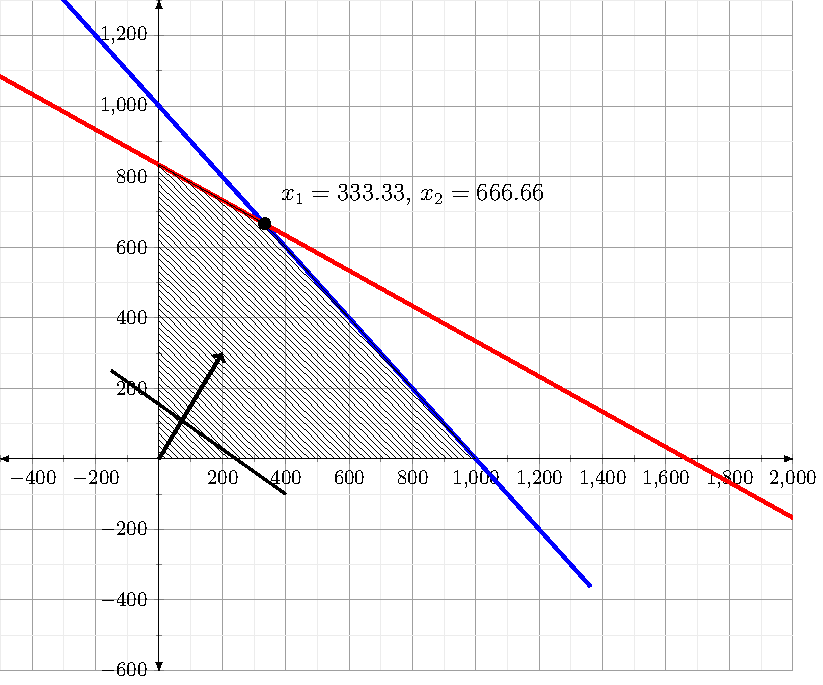
\includegraphics[width=0.8\linewidth]{plot.pdf}
\caption{Hình minh hoạ bài toán}
\end{figure}



\section{Phương pháp Gomory}
\subsection{ Giới thiệu về phương pháp Gomory}
Ta xét bài toán tối ưu nguyên dạng chính tắc:\\
\begin{equation}\label{BTNchinhtac}
     \begin{split}
          & {\rm{Min}} \langle c,x \rangle\\
          \rm{s.t} &\left\{\begin{split}
            & Ax= b,\\
           & x_j \ge 0, j=1,2,...,n.\\
            & x_j \text{nguyên}, j=1,2..,n_1 (n_1\le n).\\
           \end{split}\right.
       \end{split}
   \end{equation}
   Ta gọi:\\
   $(L^N,C)$ là bài toán tối ưu nguyên.\\
$L^N$ là miền xác định của bài toán.\\
$X(L^N,C) $ là phương án tối ưu.\\
   Ta có thể xem các bài toán tối ưu nguyên thành các trường hợp sau:\\
   1) Bài toán tối ưu nguyên hoàn toàn và giá trị hàm mục tiêu nguyên.\\
   2) Bài toán tối ưu nguyên hoàn toàn và giá trị mục tiêu không nguyên.\\
   3) Bài toán tối ưu nguyên bộ phận và giá trị hàm mục tiêu nguyên.\\
   4) Bài toán tối ưu nguyên bộ phận và giá trị hàm mục tiêu không nguyên\\
   Do trường hợp thứ nhất có thể được phát triển từ trường hợp thứ hai, trường hợp thứ ba có thể phát triển được từ trường hợp thứ tư. Do đó, ở đây chúng tôi chỉ khảo sát trên bài toán ở dạng thứ hai và thứ tư.\\
\subsection{ Tư tưởng về phương pháp cắt}
Do không thể tìm nghiệm nguyên bằng cách làm tròn nghiệm từ một bài toán tối ưu thông thường. Vậy còn cách nào tìm nghiệm nguyên mà có thể liên hệ với bài toán tối ưu thông thường hay không? Có vài ý tưởng như sau:\\

\begin{dl}
   Giả sử $L$ là một đa diện lồi,$L^N$ là tập các điểm nguyên của nó, 
$R\equiv V(L^N)$ là bao lồi tuyến tính của tập các điểm nguyên, khi đó:\\

     1) $R\equiv V(L^N)$ là một đa diện nguyên (các đỉnh là điểm nguyên).\\
     2) $R^N=L^N$.\\
    3) Tập $R^\ast$ các phương án chấp nhận được của đa diện $R$ chứa trong $R^N$:\\
    $$R^{\ast} \subseteq R^N$$.\\
\end{dl}
\begin{hq}
     Giả sử $X(R,C)$  là phương án tựa tối ưu của bài toán  $(R,C)$, khi đó
$X(R,C)$ cũng là phương án tối ưu của bài toán  $(L^N,C)$. Vì vậy để giải bài toán quy hoạch tuyến tính nguyên $(L^N,C)$ ta đi giải bài toán $(R,C)$.\\
\end{hq}
\begin{dl}
 Giả sử $L$ là một đa diện lồi, $U$ là một đa diện lồi nguyên và $U^N= L^N$, khi đó :
 $$U = R = V(L^N)$$
    \end{dl}
\begin{vd}Minh họa\\
\begin{tabular}{|c|c|c|}
    \hline
     BÀI TOÁN $(L^N,C)$  & BÀI TOÁN $(L,C)$& BÀI TOÁN $(R\equiv V(L^N,C)$  \\
     \hline
       $Max (x_1
+x_2)$  & $Max (x_1+x_2) $ &$Max (x_1+x_2)$ \\
$2x_1+11x_2\le 38$ & $2x_1+11x_2 \le 38$  \quad (a) & $x_2\le 3$\\
$x_1+x_2\le 7$ &$x_1+x_2\le 7$\quad (b) & $x_1+x_2\le 5$\\
$4x_1-5x_2\le 5$ & $4x_1-5x_2\le 5$\quad (c) & $x_1-x_2\le 1$\\
$x_j\ge 0$ & $x_j\ge 0$ & $x_j\ge 0$\\
$x_j$ nguyên & &\\
\hline 
$Max= 5$& $Max=7$ &$Max=5$\\
Tối ưu là 2 điểm & Tối ưu là một đoạn & Tối ưu là đoạn\\
$(2;3);(3;2)$&$[(\frac{13}{3},\frac{8}{3}); (\frac{40}{9};\frac{23}{9})]$&$[(2;3);(3;2)]$\\
\hline
    \end{tabular}
\begin{figure}[h]
\centering
\includegraphics[width=0.8\linewidth]{ảnh 1.pdf}
\end{figure}    
\end{vd}
Qua các định lý và hệ quả trên, đã từng có ý tưởng tìm nghiệm của bài toán tối ưu có miền xác định là một bao lồi $R$ để giải bài toán tối ưu nguyên với miền xác định $L^N$. Tuy nhiên, việc tìm được một bao lồi $R$ để thiết lập bài toán lại là một vấn đề khó giải quyết. Do đó, cần có một thuật toán khác hữu hiệu hơn.\\ 
\begin{itemize}
    \item \textbf{Khái niệm lát cắt đúng}
    Giả sử bài toán $(L^N,C)$ là bài toán quy hoạch nguyên nào đó và phương án tựa tối 
ưu của bài toán quy hoạch tuyến tính tương ứng $X(L,C)$ không thoả mãn điều kiện 
nguyên, tức là $X(L,C) \notin  L^N$. Khi đó bất đẳng thức:
    $$\sum _j a_jx_j \le \beta$$\label{latcat}\\
    được gọi là lát cắt đúng nếu thỏa mãn hai điều kiện:\\
    1) Điều kiện cắt: $x$ không thỏa mãn điều kiện \eqref{latcat}, tức là $Ax > \beta$.\\
    2) Điều kiện đúng: nếu $X(L,C)$ là phương án của bài toán tối ưu nguyên thì $X(L,C)$ thỏa mãn điều kiện \eqref{latcat}, tức là 
 $L^N \subset \{X\mid aX\le \beta\}$.\\
    Nói cách khác, lát cắt thêm vào sẽ không cắt đi một phương án nguyên nào của bài toán.\\
    
    
    \begin{figure}[h]
        \centering
        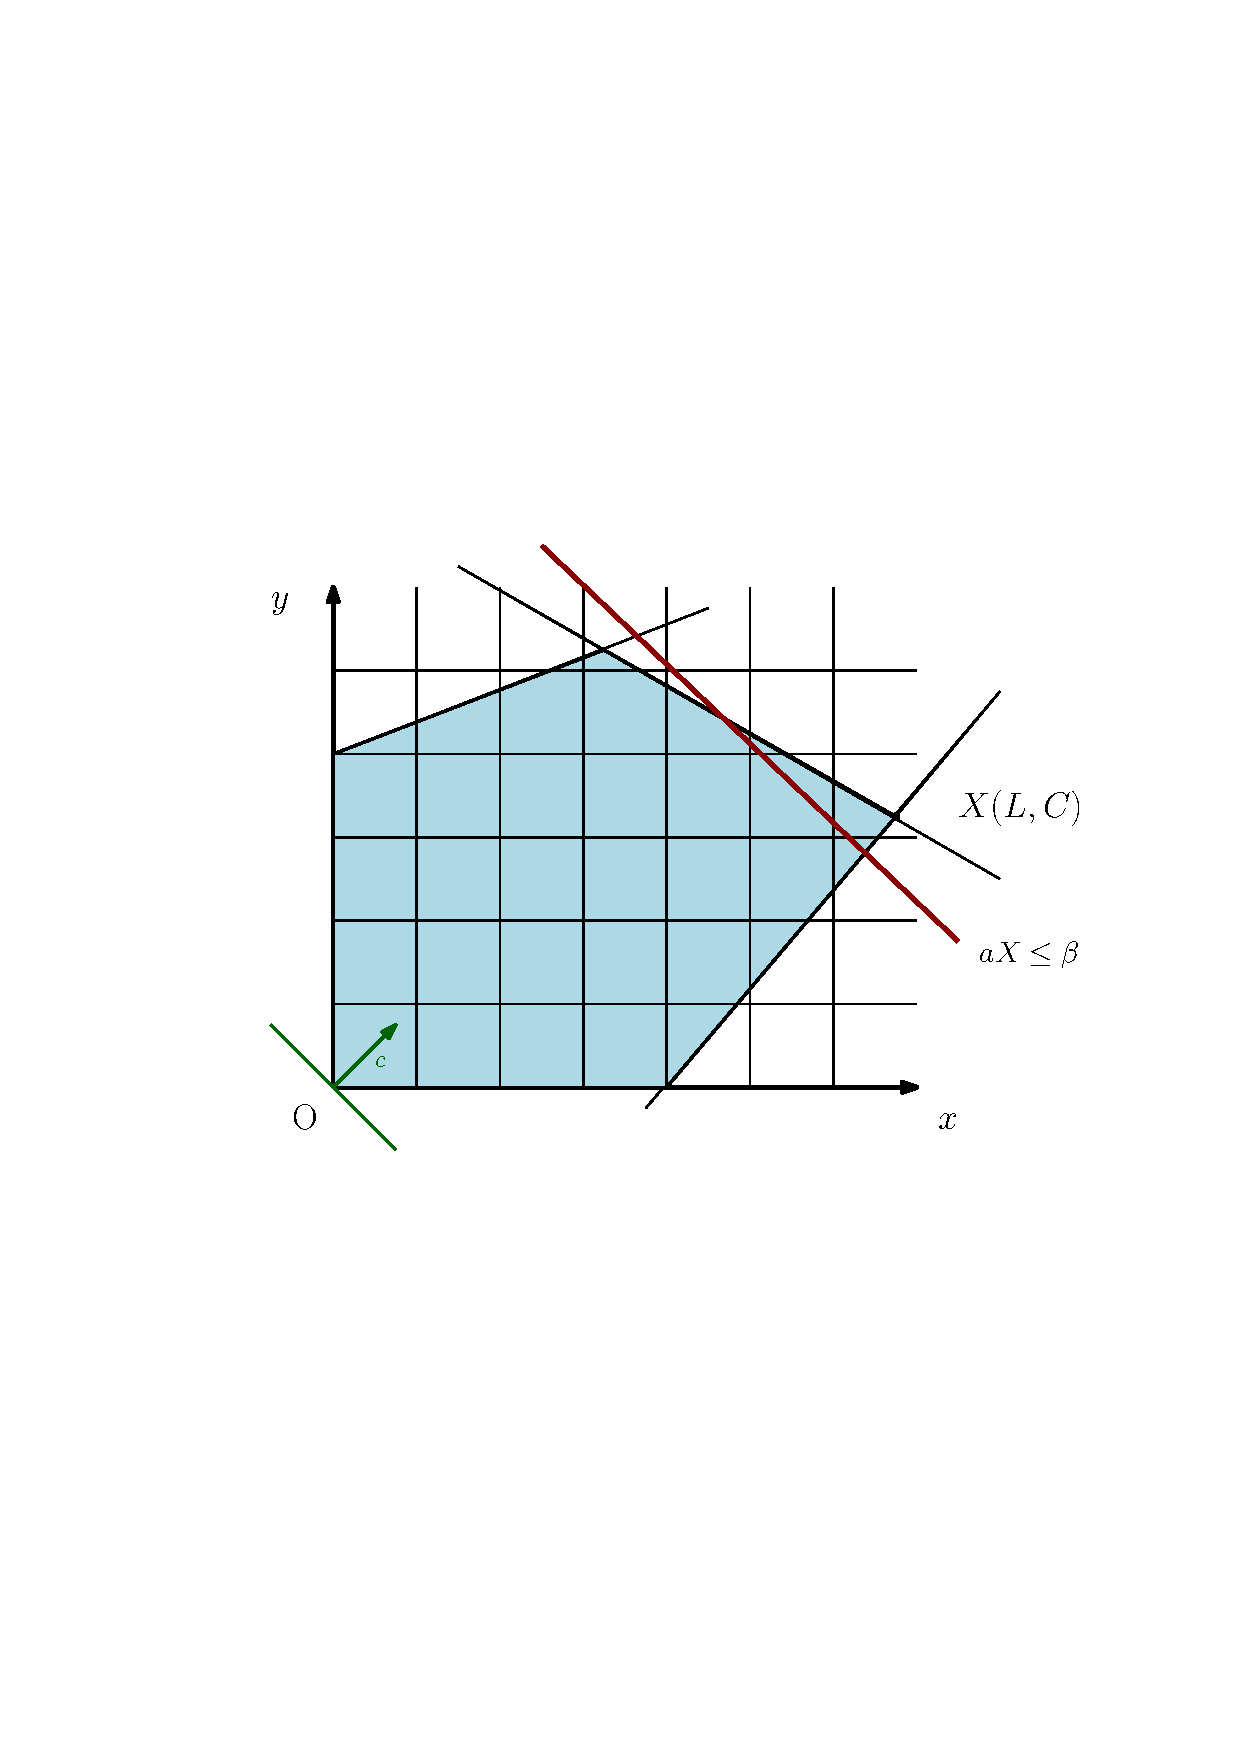
\includegraphics[width=0.8\linewidth]{anh2.pdf}
       
    \end{figure}
    \newpage
\item \textbf{Tư tưởng phương pháp cắt của Danzig}
    
    Việc giải một bài toán $(L^N,C)$ là một quá trình gồm nhiều bước:\\
a) Ở bước thứ $r$,  giải bài toán bài toán quy hoạch tuyến tính phụ 
 $(L_r,C), r = 0,1,... 
… \text{với}   L_0=L $\\
b) Tập các điểm  nguyên của tất cả các đa diện lồi là như nhau:
$$L_0^N=L_1^N=L_2^N=...=L_r^N=.......$$\\
Do đó, nếu phương án tối ưu $X(L_r,C)$ của bài toán thoả mãn $(L_r,C)$ điều kiện 
nguyên thì nó cũng là phương án tối ưu $X(L_0^N,C)$ của bài toán xuất phát $(L_0^N,C)$ và quá trình kết thúc.\\
c)  Nếu $X(L_r,C)$ không thoả mãn điều kiện nguyên thì $X(L_r,C)$ không phải là 
phương án của bài toán $X(L_{r+1},C)$, tức là $X(L_r,C)\notin L_{r+1}$.\\Chuyển từ bước $r$ sang bước $r+1$, tức là chuyển từ bài toán $(L_r,C)$ sang 
 $(L_{r+1},C)$ khi $X(L_r,C)$ không nguyên được thực hiện nhờ một lát cắt đúng $a_rx \le \beta_r$\\
Việc bổ sung lát cắt này vào ràng buộc của bài toán $(L_r,C)$ sẽ chuyển đa diện lồi $L_R$ thành $L_{r+1}$.\\
    
\end{itemize}
\begin{nx}\label{nx2.1}
    Phương pháp cắt có hai việc: xấp xỉ tuyến tính đúng nhiều bước đối với bài toán tối ưu nguyên và chuyển từ bước này sang bước khác bằng một lát cắt đúng. Ở đây tồn tại ba vấn đề cần giải quyết: xây dựng một lát cắt đúng, đảm bảo được tính hữu hạn của các bước lặp trong quá trình giải và số lượng lát cắt đúng không được tăng mãi.
\end{nx}
\subsection{ Thuật toán Gomory cho bài toán tối ưu nguyên hoàn toàn}
Ở phần này, chúng tôi sẽ trình bày về thuật toán và tính hữu hạn của thuật toán Gomory đối với bài toán tối ưu nguyên hoàn toàn và giá trị hàm mục tiêu không nguyên.Thuật toán này sẽ giải quyết được cả ba vấn đề nêu ở Nhận xét \eqref{nx2.1} một cách hiệu quả.\\
\subsubsection{Cơ sở lý thuyết}
Ta xét bài toán tối ưu nguyên hoàn toàn:\\
\begin{equation}\label{Gomory1}
     \begin{split}
          & {\rm{Max}} \langle c,x \rangle\\
          \rm{s.t} &\left\{\begin{split}
            & Ax= b,\\
           & x_j \ge 0, j=1,2,...,n.\\
            & x_j \text{nguyên}, j=1,2..,n.\\
           \end{split}\right.
       \end{split}
   \end{equation}
    Giả sử $X(L,C)$ là phương án  tối ưu của bài toán $(L,C)$, từ đó ta có thể biểu diễn các biến qua Các biến phi cơ sở:\\
   \begin{equation}\label{2.4}
       x_{i}=x_{i0} + \sum_{j \in N} x_{ij}(-x_j), i=\overline{0,m}.
   \end{equation}
    Giả sử $x$ là một số thực, ký hiệu $[x]$ là phần nguyên, (số nguyên lớn nhất không vượt quá $x), \{x\}=x-[x]$ là phần lẻ.\\
    VD: $[-1.3]=-2, {-1.3}=0.7$.\\
    \begin{dl}
        Giả sử $X(L,C)$ có $x_{i0}$ không nguyên với $1\le i\le n$ và:\\
        1)\begin{equation}\label{2.5}
            z_i\equiv z_i(X)= -\{x_{i0}\} + \sum_{j \in \mathbb {N} }(-\{x_{ij}\})(-x_{j}), i=\overline{1,n}.
        \end{equation} \\
        2) $x$ là phương án của bài toán $(L^N,C)$.\\
        Khi đó:\\
        
        a) \begin{equation}\label{2.6}
            z_i \hspace{0.1cm} \text{nguyên}
        \end{equation}
        
        b) \begin{equation}\label{2.7}
            z_i \ge 0
        \end{equation}
        \end{dl}
        \begin{cm}
            a) Từ \eqref{2.4} ta có $x_i= [x_{i0}] + \{x_{i0}\}+\underset{j \in \mathbb {N} }{ \sum}([x_{ij}]+\{x_{ij}\})(-x_{j}) $\\
    Kết hợp với \eqref{2.5} ta có $z_i= -x_i +      \underset{j \in \mathbb {N} }{ \sum}[x_{i0}] + ([x_{ij}])(-x_{ij}) $\\
    Do $x_i,x_j$ nguyên nên suy ra $z_i$ nguyên.\\
    \vspace{1cm}
    b) Giả sử rằng $z< 0$ từ \eqref{2.5} ta có:\\
    $z_i \equiv z_i (x)= -\{x_{i0}\} + \underset{j \in \mathbb {N} }{ \sum}(-\{x_{ij}\})(-x_{j})$.\\
    Vì $ {-}\{x_{i0}\}<-1 ; x_j \ge 0  $ và  $ \{x_{ij}\} \in  [0,1)$  nên $ -1<z_i<0$ , tức là $z_i$ không nguyên.\\
Điều này mâu thuẫn với chứng minh câu a), do đó $z_i \ge 0$ .
        \end{cm}
    \begin{hq}
        Giả sử $X(L,C)$ không thoả mãn điều kiện nguyên, như vậy đối 
với $i$ nào đó $(1\le i \le 0) \hspace{0.1cm} x_{i0}$ không nguyên . Khi đó các hệ thức \eqref{2.5}  và \eqref{2.7} xác định một lát cắt đúng.
    \end{hq} 
    \begin{cm}
         a) Mọi phương án của bài toán $(L^N,C)$ đều thoả mãn \eqref{2.5} và \eqref{2.7} (trong chứng 
minh định lý), do đó điều kiện đúng của lát cắt được thoả mãn. \\
b) Đặt vào \eqref{2.5} phương án tối ưu không nguyên $X(L,C)$. Do $x_j (L,C)=0$, $j \in \mathbb {N}$ , 
suy ra $z_i(X(L,C)= -\{ x_{i0}\} +0 \le 0 $ , trái với \eqref{2.7}, tức là điều kiện cắt thoả mãn.\\
    \end{cm}
    \textbf{Dấu hiệu bài toán không có lời giải:}\\
    -Nếu bài toán $(L,C)$ không có lời giải vì hàm mục tiêu không bị chặn trên khúc lồi $L$ thì thuật toán Gomory không áp dụng được.\\
-Thuật toán cũng không áp dụng được cho trường hợp bài toán $(L,C)$ có lời giải nhưng $l-\text{bài toán} \overline{(L,C)}$ không có lời giải. Điều đó dường như là tập hợp các phương án tối ưu của bài toán $(L,C)$ khác trống nhưng không bị chặn.\\
-Về sau ta sẽ giả thiết:\\
1) Hàm mục tiêu $x_0\equiv CX$ bị chặn trên L.\\
2) Nếu tập hợp các phương án tối ưu của $(L,C)$ khác trống thì nó phải bị chặn, tức là nếu bài toán$(L,C)$ giải được thì bài toán $(L,C)$ cũng giải 
được.\\

\begin{figure}[h]
\centering
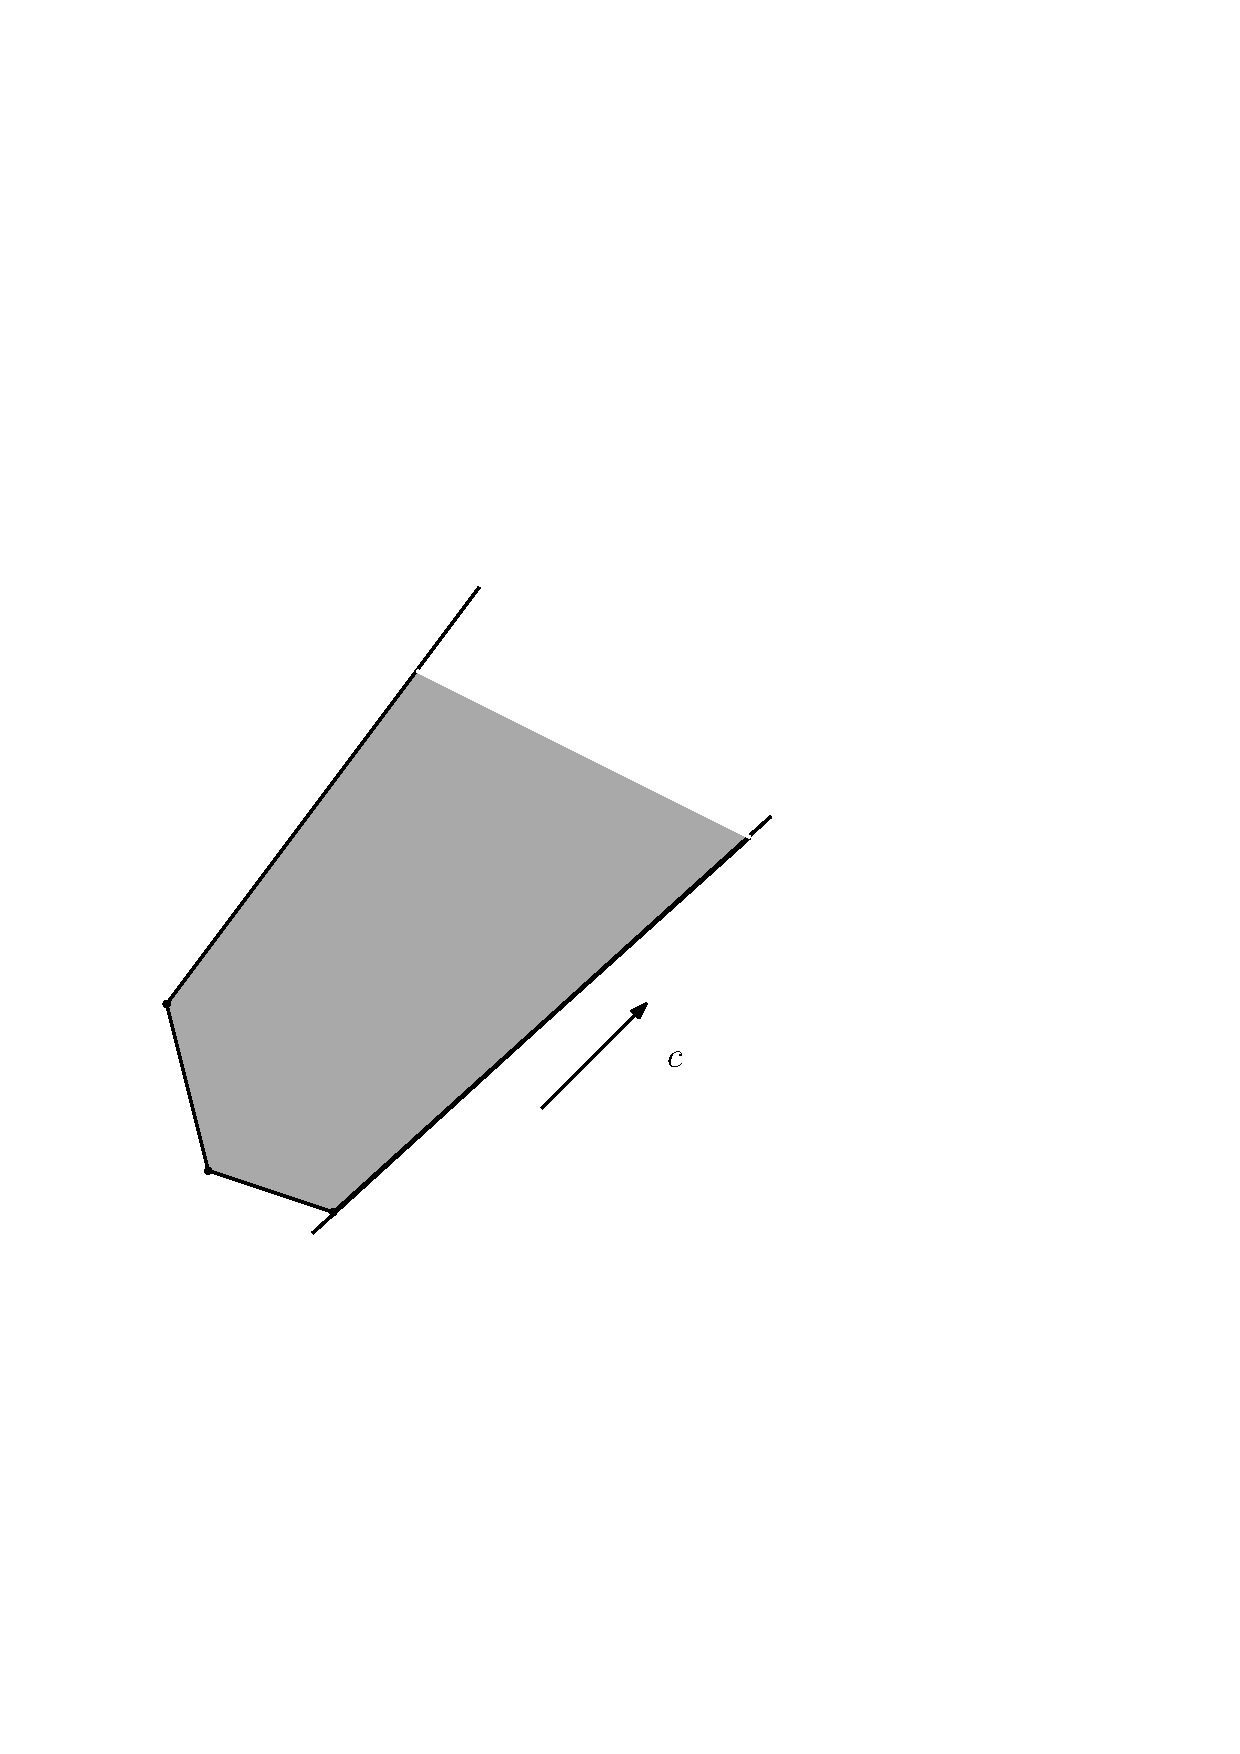
\includegraphics[width=0.4\linewidth]{anh3.pdf}
\caption{$\overline{(L,C)}$ không có lời giải}
\end{figure}
\subsubsection{ Thuật toán}

\textbf{Bước 1:}\\
Giải bài toán $(L,C)\equiv(L_0,C)$ đã cho bằng phương pháp đơn hình đối ngẫu.\\
-Nếu bài toán $(L_0,C)$ không giải được thì bài toán $(L^N_0,C)$ cũng không giải được.\\
- Nếu bài toán $(L_0,C)$ giải được và $X(L_,C)$ thỏa mãn điều kiện nguyên thì nó cũng là phương án tối ưu của bài toán $(L^N_0,C)$, còn nếu không giải được thì chuyển sang bước 2.\\

\textbf{Bước 2:}
Chọn dòng đầu tiên ứng với thành phần không nguyên:\\
$k=min\{i\|i\in \{1,...,n\},x_{i0}^r \text{không nguyên}\}$ và xây dựng lát cắt đúng:\\
$$   \begin{cases}\label{latcat}
    x_{n+r+1}= -\{x_{k0}^r\} + \sum_{j\in N_r}(-\{x_{kj}^r\} )(-x_j)\\
    x_{n+r+1} \ge 0\\
    x_{n+r+1} \hspace{0.1cm} \text{nguyên}
\end{cases}$$
Ta thêm lắt cắt này vào bảng đơn hình $T_r$, sau đó tiếp tục thực hiện các bước tính toán theo thuật toán đơn hình đối ngẫu từ vựng cho bài toán $(L^N_{r+1}$.\\

\textbf{Bước 3:}
Sau khi tính toán với lát cắt nếu được phương án tối ưu thỏa mãn điều kiện nguyên thì thuật toán dừng lại. Nếu không thỏa mãn thì quay lại bước 2 cứ lần lượt như vậy thực hiện các bước lặp $r \ge 0$ cho đến khi thỏa mãn điều kiện.
\textbf{Lưu ý:}\\
Để tránh cho bảng đơn hình không bị có số dòng và cột không xác định, mỗi khi biến phụ tương ứng với lát cắt bị đưa vào cơ sở thì cột tương ứng của nó cũng được xóa khỏi bảng đơn hình.
\subsubsection{Tính hữu hạn của thuật toán:}
\begin{dl}
Giả sử có các điều kiện sau:\\
1) Tính nguyên của hàm mục tiêu $x_0\equiv CX$ được đảm bảo và $x_0$ được xét khi chọn dòng xây dựng lát cắt đúng.\\
2) Một trong các khẳng định sau là đúng:\\
i) Hàm mục tiêu $x_0$ bị chặn dưới trên $L_0$.\\ 
ii) Bài toán $(L_0^N,C)$ có ít nhất một phương án $X'$.\\
 Khi đó thuật toán Gomory thứ nhất kết thúc sau một số hữu hạn bước lặp lớn.
 \end{dl}
 Để chứng minh định lý ta chứng minh các bổ đề trước.\\
 Giả sử
$ X\overline{(L_r,C)}\equiv X^r \equiv (x_0^r, x_1^r,x_2^r,..x_n^r) $ . Kí hiệu $\overline{X^r}$  
là giả phương án ứng với bảng $\overline{T_r}$  nhận được từ bảng $T_r$ sau khi loại khỏi cơ sở $x_{n+r+1}$  và xoá dòng tương ứng .\\
 \begin{bd}
     Ta có $X^r > \overline{X^r} \ge \overline{X^ {r+1}}$.\\
\textbf{Chứng minh: }Bất đẳng thức đầu tiên suy ra từ công thức biến đổi bảng đơn hình và tính $l$-chuẩn của bảng đơn hình (cột đầu tiên của $T_r$ được tính theo công thức $R^r_0-\dfrac{(- \{x_{k0}^r\})}{(-\{x_{kl}^r\})} . R^r_l$; $R^r_l$ có số đầu tiên khác $0$ là dương). Bất đẳng thức thứ hai là do cột $0$ giảm khi dùng phương pháp đơn hình đối ngẫu từ vựng.\\
    
 \end{bd}
  \begin{bd} Các số $x_{i} ^r (i=0,1,...,n)$ bị chặn dưới.\\
    \textbf{Chứng minh} Với $i=1,...,n$ điều đó suy ra từ điều kiện không âm $x_j \ge 0 (j=1,...,n)$. Với $i=0$ (điều đó suy ra từ điều kiện 2 của định lý 2.4). Thật vậy, nếu i) là đúng thì bổ đề 2.2 hiển nhiên đúng. Nếu điều kiện ii) được thỏa mãn thì $X^{r} \ge X^{'}$ suy ra $x^{r} _0 \ge x_0 ^{'}$.
        
    \end{bd}
    \begin{bd}
        Nếu $X^r$ không thỏa mãn điều kiện nguyên và $x_p^r \equiv x_{p0}^r$ không nguyên thì:\\
        $(x_0^r,x_1^r,...,x_{p-1}^r, [x_p^r])\ge (\overline{x^r_0},...,\overline{x^r_p})$.\\
        \textbf{Chứng minh}\\
    Giả sử $k=min\{i|i \in \{0,1,...,n\},x_{i0}^r \text{không nguyên} \}$, suy ra $k\ge p$.Giả sử:\\
    $\dfrac{R_l^r}{\{x_{kl}^r\}} =lex min \{\dfrac{R_j^r}{\{x_{kj}^r\}}|j \in N_r,\{x_{kj}^r\} \ne 0\} $\\
(dòng quay là lát cắt mới thêm) và $h(R_l^r) = min \{i|i \in (0,1,...,n);x_{il}^r\ne 0 \}$ (hàng đầu tiên của cột $R_l$ có hệ số $\ne 0$, cụ thể là $x_{hl}^r \ge 0$ do $R_l^r >0$).\\
Vì $\{x_{kl}^r\} \ne 0 \rightarrow h(R_l^r)\le k\le p$. Có hai khả năng xảy ra:\\
1) $h(R_l^r) \equiv q <p$.\\
2) $h(R_l^r) \equiv q =p$.\\
Trong trường hợp 1) theo quy tắc của $l$-phương pháp $\overline{x_q^r} < x_q^r $ vì\\
$\overline{x_q^r}= x_q^r- \frac{\{x^r_{k0}\}}{\{x_{kl}^r\}}x_{ql}^r < x ^r_q $ (do $x_{ql}^r >0 )$, bổ đề được chứng minh.
Nếu trường hợp 2) ta có $h(R_l^r)\equiv=k=$. Vì vậy $\overline{x^r_{i0}} = x^r_{i0}$ với $i<k= h(R^r_l)$ ( $h$ là chỉ số đầu tiên, $x_{hl}^r$ khác không) và $\overline{x^r_{k0}}= x^r_{k0}- \frac{\{x_{k0}^r\}}{\{x_{kl}^r\}}x_{kl}^r$.\\
Vì $x_{kl}^r=X_{hl}^r >0$, nên $x_{kl}^r \ge \{x_{kl}^r\}$. Từ đó ta có:\\
$\overline{x_{k0}^r} < x_{k0}^r - \{x_{k0}^r\}= [x_{k0}^r]$.\\
Do $k=p$ nên bổ đề được chứng minh.\\
    \end{bd}
    \textbf{Chứng minh định lí 2.4}\\
    Giả sử
    \begin{equation}\label{2.8}
      X^0,X^1,...,X^r,...\text{vô hạn}\\   
    \end{equation}
    Khi đó theo bổ đề 2.1 và 2.2 tồn tại $i_0, 0 \le i_0 \le n$ tồn tại $r_0 \ge 0$ và một dãy vô hạn:\\
    \begin{equation}\label{2.9}
        r_1<r_2<...,r_v<...(r_1>r_0)
    \end{equation}\\
    sao cho ta có:\\
   \begin{equation}\label{2.10}
       x_i^{r+1}=x_i^r; r \ge r_0; 0\le i\le i_0-1
   \end{equation} 
    \begin{equation}\label{2.11}
        x_{i_0}^{r_v+1} <x_{i_0}^{r_v}, (v=1,2,...)
    \end{equation}  \\
    Từ bổ đề 2.1 và \eqref{2.9} ta có\\
    \begin{equation}\label{2.12}
        x_{i_0}^{r+1} \le x_{i_0}^r, r\ge r_0
    \end{equation}\\
    Từ \eqref{2.11} và (\eqref{2.12} và bổ đề 2.1, suy ra tồn tại số $r' >r_0$ và các số nguyên $z_0$ và $z_0+1$ sao cho:\\
    \begin{equation}\label{2.13}
        z_0<x_{i_0}^r< z_0+1 (r \ge r')
    \end{equation}
    Từ \eqref{2.12} và \eqref{2.13} và bổ đề 2.3 suy ra $x_{i_0}^{r+1}\le \overline{x_{i_0}^r}\ge [x_{i_0}^r]=z_0$. Điều này mâu thuẫn với \eqref{2.13}.
    Định lí được chứng minh.
    \subsubsection{Ví dụ}
    \begin{equation*}
        \begin{split}
         &x_1+4x_2 \longrightarrow Max \\
        & \left\{\begin{split}
            & 2x_1+4x_2 \le 7\\
            & 10x_1+3x_2\le 15\\
            & x_1,x_2 \ge 0\\
            & x_1,x_2 \text{nguyên}\\
        \end{split}\right.
    \end{split}
    \end{equation*}
    Ta đưa bài toán về dạng chính tắc. Ta được bài toán mở rộng:\\
    \begin{equation*}
        \begin{split}
         &x_1+4x_2 \longrightarrow Max \\
        & \left\{\begin{split}
            & 2x_1+4x_2+x_3= 7\\
            & 10x_1+3x_2+   x_4= 15\\
            & x_1,x_2,x_3,x_4 \ge 0\\
            & x_1,x_2 \text{nguyên}\\
        \end{split}\right.
    \end{split}
    \end{equation*}
    Ta lập bảng đơn hình:\\
    \begin{center}
        \begin{tabular}{|c|c|c|c|c|c|c|}
    \hline
     Cơ sở & Hệ số & PA& $x_1$ &$x_2$ &$ x_3$ &$x_4$ \\
     \hline
        $x_J$ &$c_J$ &$x_J^0$ &$1$ &$4$ &$0$ &$0$\\
        \hline
        $x_3$ &$0$ &$7$ &$2$ &$4^*$ &$1$ &$0$\\
        $x_4$ &$0$ &$15$ &$10$ &$3$ &$0$ &$1$\\
        \hline
        && $\Delta$ &$-1$ &$-4^*$ &$0$ &$0$\\
        \hline
        $x_2$ &$4$ &$7/4$ &$1/2$ &$1$ &$1/4$ &$0$\\
        $x_4$ &$0$ &$39/4$ &$17/2$ &$0$ &$-3/4$ &$1$\\
        \hline
        && $\Delta$ &$1$ & $0$ &$3$ &$0$\\
        \hline
    \end{tabular}
    \end{center}
    Ta thấy bài toán đã đạt tối ưu nhưng chưa thỏa mãn điều kiện nguyên. Do đó, ta tạo biến $x_5$ theo quy tắc lát cắt Gomory dựa trên biến $x_2$, $$\dfrac{-3}{4}= \dfrac{-1}{2}x_1 -\dfrac{1}{4}x_3 +x_5$$. Ta thêm dòng này vào bảng đơn hình.\\
    \begin{center}
        \begin{tabular}{|c|c|c|c|c|c|c|c|}
        \hline
         Cơ sở & Hệ số & PA& $x_1$ &$x_2$ &$ x_3$ &$x_4$ &$x_5$\\
        \hline
        $x_J$ &$c_J$ &$x_J^0$ &$1$ &$4$ &$0$ &$0$ &$0$\\
        \hline
        $x_2$ &$4$ &$7/4$ &$1/2$ &$1$ &$1/4$ &$0$ &$0$\\
        $x_4$ &$0$ &$39/4$ &$17/2$ &$0$ &$-3/4$ &$1$ &$0$\\
        $x_5$ &$0$ &$-3/4$ &$-1/2^*$ &$0$ &$-1/4$ &$0$ &$1$\\
        \hline
        && $\Delta$ &$1^* $ &$0$ &$1$ &$0$ &$0$\\
        \hline
        $x_2$ &$ 4$ &$1$ &$0$ &$1$ &$0$ &$0$ &$1$\\
        $x-4$ &$0$ &$-3^*$ &$0$ &$0$ &$-5^*$ &$1$ &$17$\\
        $x_1$ & $1$ &$3/2$ &$1$ &$0$ &$1/2$&$0$ &$-2$\\
        \hline
        && $\Delta$ &$0$ &$0$ &$1/2$ &$0$ &$2$\\
        \hline
        $x_2$ &$4$ &$1$ &$0$ &$1$ &$0$ &$0$ &$1$\\
        $x_3$ &$0$ &$3/5$ &$0$ &$0$ &$1$ &$-1/5$ &$-17/5$\\
        $x_1$ &$1$ &$6/5$ &$1$ &$0$ &$1$ &$1/10$&$-3/10$\\
        \hline
        && $\Delta$ &$0$ &$0$ &$0$ &$1/10$ &$37/10$\\
        \hline
        
        \end{tabular}
    \end{center}
    Ta thêm lát cắt mới dựa trên biến $x_1$, 
     $$\dfrac{-1}{5}= \dfrac{-1}{10}x_4 +\dfrac{7}{10}x_5+x_6$$
     \begin{center}
         \begin{tabular}{|c|c|c|c|c|c|c|c|c|}
        \hline
         Cơ sở & Hệ số & PA& $x_1$ &$x_2$ &$ x_3$ &$x_4$ &$x_5$ &$x_6$\\
        \hline
        $x_J$ &$c_J$ &$x_J^0$ &$1$ &$4$ &$0$ &$0$ &$0$ &$0$\\
        \hline
        $x_2$ &$4$ &$1$ &$0$ &$1$ &$0$ &$0$ &$1$ &$0$\\
        $x_3$ &$0$ &$3/5$ &$0$ &$0$ &$1$ &$-1/5$ &$-17/5$ & $0$\\
        $x_1$ &$1$ &$6/5$ &$1$ &$0$ &$1$ &$1/10$&$-3/10$ &$0$\\
        $x_6$ &$0$ &$-1/5$ &$0$ &$0$ & $0$ &$-1/10^*$ &$7/10$ &$1$\\
        \hline
        && $\Delta$ &$0$ &$0$ &$0$ &$1/10$ &$37/10$ &$0$\\
        \hline
        $x_2$ &$4$ &$1$ &$0$ &$1$ &$0$ &$0$ &$1$ &$0$\\
        $x_3$ &$0$ &$1$ &$0$ &$0$ &$1$ &$0$ &$-24/5$ &$-2$\\
        $x_1$ &$1$ &$1$ &$1$ &$0$ &$0$ &$0$ &$2/5$ &$1$\\
        $x_4$ &$0$ &$2$ &$0$ &$0$ &$0$ &$1$ &$-7$ &$-10$\\
        \hline
        && $\Delta$ &$0$ &$0$ &$0$ &$0$&$ 22/5$ &$1$\\
        \hline
        
         \end{tabular}
     \end{center}
     Bài toán đã đạt tối ưu đồng thời thỏa điều kiện nguyên nên ta dừng thuật toán và kết luận được $x=(x_1,x_2)=(1,1)$ và giá trị hàm mục tiêu là $5$.
\subsection{Thuật toán Gomory cho bài toán tối ưu nguyên bộ phân}
 Đối với bài toán tối ưu nguyên bộ phận ta có tất cả các lý thuyết cơ sở cũng như thuật toán tương tự như ở bài toán tối ưu nguyên hoàn toàn.Tuy nhiên, ở việc chọn dòng để hình thành lát cắt:
 $k=min\{i\|i\in \{1,...,n\},x_{i0}^r \text{không nguyên}\}$, trong đó ta chỉ xét trên các biến mà đề bài bắt buộc nguyên, và trực tiếp bỏ qua các biến không có điều kiện nguyên.
 \subsubsection{Ví dụ}
 Ta xét bài toán sau:
 \begin{equation*}
        \begin{split}
         & 4x_1+5x_2+3x_3\longrightarrow Max \\
        & \left\{\begin{split}
            & 3x_1+   +4x_3 \le 10\\
            & 2x_1+x_2+x_3 \le 7\\
            & 3x_1+4x_2+x_3 \le 12\\
            & x_1,x_2,x_3 \ge 0\\
            & x_1,x_3 \text{nguyên}\\
        \end{split}\right.
    \end{split}
    \end{equation*}
    Ta đưa bài toán về dạng chính tắc:\\
    \begin{equation*}
        \begin{split}
         &4x_1+5x_2+3x_3 \longrightarrow Max \\
        & \left\{\begin{split}
            & 3x_1+  +4x_3+x_4=10\\
            &2x_1+x_2+x_3+x_5=7\\
            &3x_1+4x_2+x_3+  x_6=12\\
            & x_1,x_2,x_3,x_4,x_4,x_6 \ge 0\\
            & x_1,x_3 \text{nguyên}\\
        \end{split}\right.
    \end{split}
    \end{equation*}
    \begin{center}
        \begin{tabular}{|c|c|c|c|c|c|c|c|c|}
        \hline
         Cơ sở & Hệ số & PA& $x_1$ &$x_2$ &$x_3$ &$x_4$ &$x_5$ &$x_6$  \\
         \hline
          $x_J$& $c_J$ &$x_J^0$ &$4$ &$5$ &$ 3$ &$0$ &$0$ &$0$\\
          \hline
          $x_4$ &$0$ &$10$ &$3$ &$0$ &$4$ &$1$ &$0$ &$0$\\
          $x_5$ &$0$ &$7$ &$2$ &$1$ &$1$ &$0$ &$1$ &$0$\\
          $x_6$ &$0$ &$12$ &$3$ &$4^*$ &$1$ &$0$ &$0$ &$1$\\
          \hline
          &&$\Delta$ &$-4$ &$-5$ &$-3$ &$0$ &$0$ &$0$\\
          \hline
      \end{tabular}
    \end{center}    
    \begin{center}
        \begin{tabular}{|c|c|c|c|c|c|c|c|c|}
        \hline
          Cơ sở & Hệ số & PA& $x_1$ &$x_2$ &$x_3$ &$x_4$ &$x_5$ &$x_6$  \\
         \hline
          $x_J$& $c_J$ &$x_J^0$ &$4$ &$5$ &$ 3$ &$0$ &$0$ &$0$\\
          \hline    
          $x_4$ & $0$ &$10$ &$3$ &$0$ &$4^*$ &$1$ &$0$ &$0$ \\
          $x_5$ &$0$ &$4$ &$5/4$ &$0$ &$3/4$ &$0$ &$1$ &$-1/4$\\
          $x_2$ &$5$ &$3$ &$3/4$ &$1$ &$1/4$ &$0$ &$0$ &$1/4$\\
          \hline
          &&$\Delta$ &$-1/4$ &$0$ &$-3^*$ &$0$ &$0$ &$5/4$\\
          \hline
          $x_3$ &$3$ &$5/2$ &$3/4$ &$0$ &$1$ &$1/4$ &$0$ &$0$\\
          $x_5$ &$0$ &$17/8$ &$11/16$ &$0$ &$0$ &$-3/16$ &$0$ &$-1/4$\\
          $x_2$ &$5$ &$19/8$ &$9/16$ &$1$ &$0$ &$-1/16$ &$1$ &$1/4$\\
          \hline
          &&$\Delta$ &$17/16$ &$0$ &$0$ &$7/16$ &$0$ &$5/4$\\
          \hline
         \end{tabular}
    \end{center}
    Lúc này bài toán đạt tối ưu nhưng chưa thỏa điều kiện nguyên, ta xét biến $x_3$ để tạo lát cắt Gomory, bỏ qua $x_2$ vì đề bài chỉ yêu cầu $x_1,x_3$ phải nguyên.
    $$\dfrac{-1}{2}=\dfrac{-3}{4}x_1 -\dfrac{1}{4}x_4 +x_7$$.
    \begin{center}
        \begin{tabular}{|c|c|c|c|c|c|c|c|c|c|}
        \hline
         Cơ sở & Hệ số & PA& $x_1$ &$x_2$ &$x_3$ &$x_4$ &$x_5$ &$x_6$ &$x_7$ \\
         \hline
          $x_J$& $c_J$ &$x_J^0$ &$4$ &$5$ &$ 3$ &$0$ &$0$ &$0$ &$0$\\
          \hline
           $x_3$ &$3$ &$5/2$ &$3/4$ &$0$ &$1$ &$1/4$ &$0$ &$0$ &$0$\\
          $x_5$ &$0$ &$17/8$ &$11/16$ &$0$ &$0$ &$-3/16$ &$0$ &$-1/4$ &$0$\\
          $x_2$ &$5$ &$19/8$ &$9/16$ &$1$ &$0$ &$-1/16$ &$1$ &$1/4$ &$0$\\
          $x_7$ &$0$ &$-1/2$ &$-3/4$ &$0$ &$0$ &$-1/4^*$ &$0$ &$0$ &$1$\\
          \hline
          &&$\Delta$ &$17/16$ &$0$ &$0$ &$7/16$ &$0$ &$5/4$ &$0$\\
          \hline
          $x_3$ &$3$ &$2$ &$3/4$ &$0$ &$1$ &$0$ &$0$ &$0$ &$1$\\
          $x_5$ &$0$ &$5/2$ &$5/4$ &$0$ &$0$ &$0$ &$1$ &$-1/4$ &$-3/4$\\
          $x-2$ &$5$ &$5/2$ &$3/4$ &$1$ &$0$ &$0$ &$0$ &$1/4$ &$-1/4$\\
          $x_4$ &$0$ &$2$ &$3^*$ &$0$ &$0$ &$1$ &$0$ &$0$ &$-4$\\
          \hline
          &&$\Delta$&$-1/4$ &$0$ &$0$ &$0$ &$0$ &$5/4$ &$7/4$\\
          \hline
          \end{tabular}
    \end{center}    
    \begin{center}
        \begin{tabular}{|c|c|c|c|c|c|c|c|c|c|}
        \hline
          Cơ sở & Hệ số & PA& $x_1$ &$x_2$ &$x_3$ &$x_4$ &$x_5$ &$x_6$ &$x_7$ \\
         \hline
          $x_J$& $c_J$ &$x_J^0$ &$4$ &$5$ &$ 3$ &$0$ &$0$ &$0$ &$0$\\
          \hline
          $x_3$ &$3$ &$2$ &$0$ &$0$ &$1$ &$0$ &$0$ &$0$ &$1$\\
          $x_5$ &$0$ &$5/3$ &$0$ &$0$ &$0$ &$5/12$ &$1$ &$-1/4$ &$11/2$\\
          $x_2$ &$5$ &$2$ &$0$ &$1$ &$0$ &$-1/4$ &$0$ &$1/4$ &$3/4$\\
          $x_1$ &$4$ &$2/3$ &$1$ &$0$ &$0$ &$1/3$ &$0$ &$0$ &$-4/3$\\
          \hline
          &&$\Delta$ &$0$ &$0$ &$0$ &$1/12$ &$0$ &$5/4$ &$17/12$\\
          \hline
        \end{tabular}
    \end{center}
    Ta xét $x_1$ và lập lát cắt mới, $\dfrac{-2}{3}= \dfrac{-1}{3}x_4 +\dfrac{1}{3}x_7+x_8$.
    \begin{center}
        \begin{tabular}{|c|c|c|c|c|c|c|c|c|c|c|}
        \hline
          Cơ sở & Hệ số & PA& $x_1$ &$x_2$ &$x_3$ &$x_4$ &$x_5$ &$x_6$ &$x_7$&$x_8$ \\
         \hline
          $x_J$& $c_J$ &$x_J^0$ &$4$ &$5$ &$ 3$ &$0$ &$0$ &$0$ &$0$ &$0$\\
          \hline
           $x_3$ &$3$ &$2$ &$0$ &$0$ &$1$ &$0$ &$0$ &$0$ &$1$ &$0 $\\
          $x_5$ &$0$ &$5/3$ &$0$ &$0$ &$0$ &$5/12$ &$1$ &$-1/4$ &$11/2$ &$0$\\
          $x_2$ &$5$ &$2$ &$0$ &$1$ &$0$ &$-1/4$ &$0$ &$1/4$ &$3/4$ &$0$\\
          $x_1$ &$4$ &$2/3$ &$1$ &$0$ &$0$ &$1/3$ &$0$ &$0$ &$-4/3$ &$0$\\
          $x_8$ &$0$ &$-2/3$ &$0$ &$0$ &$0$ &$-1/3^*$ &$0$ &$0$ &$1/3$ &$1$\\
          \hline
          &&$\Delta$ &$0$ &$0$ &$0$ &$1/12$ &$0$ &$5/4$ &$17/12$ &$0$\\
          \hline
          $x_3$ &$3$ &$2$ &$0$ &$0$ &$1$ &$0$ &$0$ &$1$ &$0$& $0$\\
          $x_5$ &$0$ &$5/6$ &$0$ &$0$ &$0$ &$0$ &$1$ &$-1/4$ &$71/12$ &$5/4$\\
          $x_2$ &$5$ &$5/2$ &$0$ &$1$ &$0$ &$0$ &$0$&$1/4$ &$1/2$ &$-3/4$\\
          $x_1$ &$4$ &$0$ &$1$ &$0$ &$0$ &$0$ &$0$ &$0$ &$-1$ &$1$\\
          $x_4$ &$0$ &$2$ &$0$ &$0$ &$0$ &$1$ &$0$ &$0$ &$-1$ &$-3$\\
          \hline
          &&$\Delta$ &$0$ &$0$ &$0$ &$0$ &$0$ &$5/4$ &$3/2$ &$1/4$\\
          \hline
        \end{tabular}
    \end{center}
    Ta dừng thuật toán và kết luận nghiệm của bài toán đã cho là $x=(x_1,x_2,x_3)=(0,\dfrac{5}{2},2)$ và giá trị tối ưu của hàm mục tiêu là $18.5$.

\section{Phương pháp Land-Doig (Nhánh cận)}

Vào cuối những năm 1950, một nhóm giáo viên và nhà nghiên cứu tại Trường Kinh tế Luân Đôn, gồm có Helen Makower, George Morton, Ailsa Land và Alison Doig, đã bị thu hút bởi lĩnh vực quy hoạch tuyến tính và các ứng dụng của nó. Ban đầu, Ailsa Land và Alison Doig tập trung vào các vấn đề mà ngày nay ta còn gọi là bài toán người du lịch.

Sau đó, bà chuyển dần sự chú ý sang các biến rời rạc và ứng dụng chúng vào các mô hình quy hoạch tuyến tính theo yêu cầu của Tập đoàn Dầu mỏ Anh (British Petroleum). Mặc dù không có các điều kiện công nghệ như hiện này để có thể tiếp cận tính toán điện tử nhưng bà đã tiên phong trong việc phát triển các phương pháp xử lý biến rời rạc thông qua tính toán thủ công và sử dụng máy tính thời bấy giờ. Cách tiếp cận của bà xoay quanh việc khám phá các tập lồi được xác định bởi các ràng buộc tuyến tính, sau này được công nhận là một dạng của phương pháp nhánh cận. Bà đã thành công trong việc giải quyết cả mô hình lập kế hoạch và xử lý nguyên bộ phận. Phát hiện của bà được công bố trên tạp chí Econometrica, đánh dấu một bước tiến quan trọng trong lĩnh vực tối ưu tuyến tính.

\subsection{Giới thiệu bài toán}
Trong bài toán tối ưu tuyến tính giải cho ra nghiệm nguyên, đôi lúc ta gặp trường hợp yêu cầu tất cả các nghiệm cho ra nguyên và đôi lúc chỉ yêu cầu một vài nghiệm nguyên.

Từ đó ta tập trung vào 2 loại bài toán là bài toán Tối ưu nguyên hoàn toàn và bài toán Tối ưu nguyên bộ phận.
\subsection*{Tối ưu nguyên hoàn toàn (Pure integer linear program)}
    Ta xét bài toán sau:
    \begin{equation} \label{H}
        \begin{split}
        (H) \quad & z_h=c^Tx \quad \longrightarrow Max \\
                  & \left\{\begin{split}
                    &Ax \leq  b, \\
                    &x \geq 0, \text{ nguyên} \\
                    \end{split}\right.    
        \end{split}
        \end{equation}            

    Trong đó $H$ tương ứng với hoàn toàn, $c^T=(c_1 \: c_2 \: \ldots \: c_n)$, $A$ là ma trận $m\times n$, $b=\begin{pmatrix}
        b_1 \\
        b_2 \\
        \vdots \\
        b_m
        \end{pmatrix}$, với $x\in Z^n$. Bài toán $(H)$ gọi là bài toán \textbf{Tối ưu nguyên hoàn toàn} và tập $S_h:=\{x\in Z^n_+: Ax\leq b\}$ là tập nghiệm của bài toán Tối ưu nguyên hoàn toàn.


%model_1: hoan toan
 \subsubsection*{Minh hoạ bài toán}
    \begin{equation}
        \begin{split}
        \quad & 2x_1 + 2x_2 \quad \longrightarrow Max \\
                    & \left\{\begin{split}
                    & x_1 + 3x_2 \leq 24 \\
                    & \frac{13}{3}x_1 + 2x_2 \leq 32.5 \\
                    &x_1 \geq 0, \text{ nguyên}. \\
                    &x_2 \geq 0, \text{ nguyên}. \\
                    \end{split}\right.    
        \end{split}
        \end{equation}            
Xem hình 2.3.
\begin{figure}
\center
\begin{tikzpicture}
\begin{axis}
    [
    xmin=0,xmax=10,
    ymin=0,ymax=10,
    grid=both,
    grid style={line width=.1pt, draw=darkgray!50},
    major grid style={line width=.2pt,draw=darkgray!50},
    axis lines=middle,
    minor tick num=1,
    enlargelimits={abs=0},
    samples=100,
    domain = -20:20,
    ]
    \filldraw[green, pattern=north west lines, pattern color=green, line width=2pt] (0, 0) -- (0, 8) -- (4.5, 6.5) -- (7.5, 0) -- cycle;
\end{axis}
\end{tikzpicture}  
\caption{Tập nghiệm của bài toán Tối ưu nguyên hoàn toàn}
\end{figure}

\subsection*{Tối ưu nguyên bộ phận (Mixed integer linear program)}
Ta xét bài toán sau:
\begin{equation}\label{B}
\begin{split}
(B) \quad & z_b=c^Tx+h^Ty \quad \longrightarrow Max \\
          & \left\{\begin{split}
            &Ax+Gy \leq  b, \\
            &x \geq 0, \text{ nguyên} \\
            &y \geq 0.
            \end{split}\right.    
\end{split}
\end{equation}    
Trong đó $B$ tương ứng với bộ phận, $c^T=(c_1 \: c_2 \: \ldots \: c_n)$, $h^T=(h_1 \: h_2 \: \ldots \: h_p)$, $A$ là ma trận $m\times n$, $G$ là ma trận $m\times p$, $b=\begin{pmatrix}
    b_1 \\
    b_2 \\
    \vdots \\
    b_m
    \end{pmatrix}$, với $x\in Z^n$ và $y\in R^p$.
Bài toán $(B)$ gọi là bài toán \\ \textbf{Tối ưu nguyên bộ phận} và tập $S_b:=\{(x,y)\in Z^n_+\times R^p_+: Ax+Gy\leq b\}$ là tập nghiệm của bài toán Tối ưu nguyên bộ phận.

\subsubsection*{Minh hoạ bài toán}
   \begin{equation}
        \begin{split}
        \quad & x_1 + 2x_2 \quad \longrightarrow Max \\
                    & \left\{\begin{split}
                    & 5x_1 + \frac{15}{7}x_2 \leq 20 \\
                    & -2.4x_1 + \frac{30}{7}x_2 \leq 15 \\
                    &x_1 \geq 0, \text{ nguyên}. \\
                    &x_2 \geq 0. \\
                    \end{split}\right.    
        \end{split}
        \end{equation}            
Xem hình 2.4.

\begin{figure} \label{bophan}
\center	
\begin{tikzpicture}
\begin{axis}
    [
    xmin=0,xmax=5,
    ymin=0,ymax=5,
    grid style={line width=.1pt, draw=darkgray!50},
    major grid style={line width=.2pt,draw=darkgray!50},
    axis lines=middle,
    minor tick num=1,
    enlargelimits={abs=0},
    samples=100,
    domain = -20:20,
    xmajorgrids=true,
    ]
    \filldraw[green, pattern=north west lines, pattern color=green, line width=2pt] (0, 0) -- (0, 2.5) -- (2.5, 3.5) -- (4, 0) -- cycle;
\end{axis}
\end{tikzpicture}  
\caption{Tập nghiệm của bài toán Tối ưu nguyên bộ phận}
\end{figure}

    
\subsection{Ý nghĩa của phương pháp và thuật toán Land-doig (Nhánh cận)}

Ta quan tâm bài toán sau:
\begin{equation}\label{P}
\begin{split}
(P) \quad & z_p=c^Tx+h^Ty \quad \longrightarrow Max \\
            & \left\{\begin{split}
                &Ax+Gy \leq  b, \\
                &x,y \geq 0.
            \end{split}\right.    
\end{split}
\end{equation}
Trong đó $(P)$ là bài toán tối ưu tuyến tính nguyên bộ phận $(B)$ với nghiệm thuộc tập số thực.
Bài toán $(P)$ là một bài toán \textbf{Tối ưu tuyến tính thông thường} hay gọi đơn giản là bài toán Tối ưu tuyến tính (Natural linear programming relaxation).
Tập $S_p:=\{(x,y)\in R^n_+\times R^p_+: Ax+Gy\leq b\}$ là tập nghiệm của bài toán Tối ưu tuyến tính.

Giả sử ta nhận được tập phương án tối ưu của bài toán \eqref{B} sau hữu hạn lần giải, ký hiệu $(x_b, y_b)$ và giá trị tối ưu là $z_b$ thì ta có nhận xét sau:
\begin{nx} \label{nx}
\phantom{abc}
\begin{itemize}
\item Nếu $S_b \subseteq S_p$ thì ta luôn nhận được $z_b \leq z_p$ và phương án có thể cải thiện.
\item Nếu $S_b = S_p$ thì ta nhận được $z_b = z_p$ và bài toán được giải.
\end{itemize}    
\end{nx}
Vì thế, ta chọn xử lý bài toán $(B)$ thông qua bài toán $(P)$ bằng cách cải thiện phương án thu được từ bài toán $(P)$ sao cho thoả điều kiện của bài toán $(B)$.

\subsubsection*{Ví dụ}
Cho bài toán:
        \begin{equation} \label{baitoannguyenloi}
        \begin{split}
            (B) \quad & 5.5x_1 + 2.1x_2 \quad \longrightarrow Max \\
            & \left\{\begin{array} {cccc}
            -1x_1 &+ x_2 &\leq& 2 \\
            8x_1 &+ 2x_2 &\leq& 17 \\
            x_1 &&\geq & 0, \text{ nguyên} \\
            &x_2 &\geq& 0, \text{ nguyên}. \\
            \end{array}\right.
            \Longrightarrow
            \left\{\begin{array} {ccc}
            \mathbf{x_1} & \mathbf{=}& \mathbf{1.3} \\
            \mathbf{x_2} &\mathbf{=}& \mathbf{3.3} \\
            z &=&14.08
        \end{array}\right.
        \end{split}
        \end{equation}
    Bài toán (B) có thể tiếp tục cải thiện phương án do ta có $x_1=1.3$ và $x_2=3.3$ chưa thoả điều kiện nghiệm của bài toán.



\subsubsection*{Ví dụ}
        \begin{equation} \label{baitoannguyenhet}
        \begin{split}
            (B) \quad & 3x_1 + 4x_2 \quad \longrightarrow Max \\
            & \left\{\begin{array} {cccc}
            2.5x_1 &+ \frac{15}{4}x_2 &\leq& 20 \\
            x_1 &+ \frac{5}{3}x_2 &\leq& \frac{50}{3} \\
            x_1 &&\geq &0, \\
            &x_2 &\geq& 0. \\
            \end{array}\right.
            \Longrightarrow
            \left\{\begin{array}{ccc}
            x_1 &= &5 \\
            x_2 &= &7 \\
            z& =&43
        \end{array}\right.
        \end{split}
        \end{equation}
    Bài toán được giải.

\subsection*{Phương pháp xác định cận}
Ta gọi $x_j$ với $1 \leq j \leq n$ là nghiệm thu được từ bài toán $(P)$.
\begin{dl}\label{cmnguyen}
	\phantom{}
Với mỗi $x_j \in \mathbb{R}$, tồn tại duy nhất số nguyên $k \in \mathbb{Z}$ sao cho $k \leq x_j < k+1$.
\begin{itemize}
\item Giá trị $k$ khi đó ta gọi là phần nguyên nhỏ nhất của $x_j$, ký hiệu là $\lfloor x_j \rfloor$.
\item Giá trị $k+1$ gọi là phần nguyên lớn nhất của $x_j$, ký hiệu là $\lceil x_j \rceil$.
\end{itemize}
\end{dl}

\begin{vd}
Ta có $x_1=3.3$, vậy khi đó phần nguyên nhỏ nhất của $x_1$ là $\lfloor x_1 \rfloor = 3$ và phần nguyên lớn nhất là $\lceil x_1 \rceil =4$.
\end{vd}

\subsection*{Phương pháp xử lý bài toán}

Từ ví dụ minh hoạ của hai bài toán \eqref{baitoannguyenloi} và \eqref{baitoannguyenhet}, ta thấy rằng nếu tồn tại bất kỳ $x_j$ không thuộc $\mathbb{Z}$, thì ta có thể tiếp tục cải thiện phương án cho đến khi với mọi $x_j$ thuộc $\mathbb{Z}$. 
Nếu nghiệm thu được là $x_j \notin \mathbb{Z}$, ta thiết lập được 2 bài toán con từ bài toán $(P)$ ban đầu, ký hiệu $(P_1)$ và $(P_2)$.

\begin{equation}
    \begin{split}
    (P_1) \quad & z_1=c^Tx+h^Ty \quad \longrightarrow Max \\
                & \left\{\begin{split}
                    &Ax+Gy \leq  b \\
                    &\color{blue} x_j \leq \lfloor x_j \rfloor , \\
                    &x,y \geq 0.
                \end{split}\right.    
    \end{split}
\end{equation}
Tập $S_1:=S_p \cap \{ (x,y): x_j \leq \lfloor x_j \rfloor \}$ là tập nghiệm tối ưu của bài toán con $(P_1)$.



\begin{equation}
    \begin{split}
    (P_2) \quad & z_2=c^Tx+h^Ty \quad \longrightarrow Max \\
                & \left\{\begin{split}
                    &Ax+Gy \leq  b \\
                    &\color{blue} x_j \geq \lceil x_j \rceil , \\
                    &x,y \geq 0.
                \end{split}\right.    
    \end{split}
\end{equation}
Tập $S_2:=S_p \cap \{ (x,y): x_j \geq \lceil x_j \rceil \}$ là tập nghiệm tối ưu của bài toán con $(P_2)$.

\subsection*{Điều kiện nghiệm}
Nếu tồn tại $(P_i)$ với $i=1,2$ không giải được $(S_i = \emptyset )$, ta gọi bài toán \textbf{vô nghiệm}. Giả sử $x^{(i)}$ là nghiệm tối ưu của bài toán $(P_i)$ và giá trị tối ưu là $z_i$ với $i = 1,2$. Tồn tại các trường hợp sau:
\begin{itemize}
\item Nếu $\forall x^{(i)} \in Z^n_+$, ta nói $S_i$ là tập nghiệm thoả mãn bài toán tối ưu nguyên bộ phận, $z^*_i$ là giá trị tối ưu và bài toán con $(P_i)$ được giải, ta gọi bài toán được \textbf{gọt bởi nghiệm nguyên}.
\item Nếu $\exists x^{(i)} \notin Z^n_+$ đồng thời $z_i \leq z^*_i$, ta dừng phân nhánh và bỏ qua bài toán, ta gọi bài toán được \textbf{gọt bởi cận}.
\item Nếu $\exists x^{(i)} \notin Z^n_+$ đồng thời $z_i > z^*_i$, bài toán chưa tối ưu và có thể tiếp tục cải thiện.
\iffalse
Với $x^{(i)}_{j^'}$ là nghiệm không nguyên và phân thành 2 bài toán con $P_3$ với tập nghiệm $S_l := S_i \cap \{ (x,y): x_{j^{'}} \leq \lfloor x_{j^{'}} \rfloor \}$, $P_l$ với $S_l := S_i \cap \{ (x,y): x_{j^{'}} \geq \lceil x_{j^{'}} \rceil \}$ trong đó $l=3,4$ và lặp lại quá trình.
\fi
\end{itemize}

\begin{cy}
Ta gọi $x_j^{(i)}$ là biến thứ $j$ của bài toán thứ $i$.
\end{cy}

\subsubsection*{Ví dụ minh hoạ}
    \begin{equation*}
        \begin{split}
            (P) \quad z_p= & 5.5x_1 + 2.1x_2 \quad \longrightarrow Max \\
            & \left\{\begin{array}{cccc}
            -x_1 &+ x_2 &\leq& 2 \\
            8x_1 &+ 2x_2 &\leq& 17 \\
            x_1 &&\geq& 0, \\
            &x_2 &\geq& 0. \\
            \end{array}\right. \\
        \end{split}
    \end{equation*}



    Giải bài toán bằng phương pháp đơn hình thông thường ta thu được nghiệm $x_1 =1.3$, $x_2 = 3.3$ và $z_p=14.08$ với tập nghiệm của bài toán (hình 2.5). Chọn $x_1=1.3$ để cải thiện phương án, ta thu được 2 bài toán con sau:
    \begin{figure}
	\center
    \begin{tikzpicture}
    \begin{axis}
        [
        xmin=0,xmax=3,
        ymin=0,ymax=5,
        grid style={line width=.1pt, draw=darkgray!50},
        major grid style={line width=.2pt,draw=darkgray!50},
        axis lines=middle,
        minor tick num=1,
        enlargelimits={abs=0},
        samples=100,
        domain = -20:20,
        xmajorgrids=true,
        ]
        \filldraw[blue, pattern=north west lines, pattern color=blue, line width=2pt] (0, 0) -- (0, 2) -- (1.3, 3.3) -- (2.125, 0) -- cycle;
    \end{axis}
    \end{tikzpicture}  
    \caption{Tập nghiệm của bài toán}
    \end{figure}

    \begin{equation*}
        \begin{split}
            (P_1) \quad z_1= & 5.5x^{(1)}_1 + 2.1x^{(1)}_2 \\
            & \left\{\begin{array} {cccc}
            -x^{(1)}_1 &+ x^{(1)}_2 &\leq& 2 \\
            8x^{(1)}_1 &+ 2x^{(1)}_2 &\leq& 17 \\
            \color{blue} x^{(1)}_1 && \color{blue} \leq &\color{blue} 1 \\
            x^{(1)}_1 &&\geq& 0 \\
            &x^{(1)}_2 &\geq& 0. \\
            \end{array}\right. \\
        \end{split}
    \end{equation*}
   \begin{equation*}
        \begin{split}
            (P_2) \quad z_2= & 5.5x^{(2)}_1 + 2.1x^{(2)}_2  \\
            & \left\{\begin{array} {cccc}
            -x^{(2)}_1 &+ x^{(2)}_2 &\leq &2 \\
            8x^{(2)}_1 &+ 2x^{(2)}_2 &\leq &17 \\
            \color{blue} x^{(2)}_1 &&\color{blue}\geq&\color{blue} 2 \\
            x^{(2)}_1 &&\geq& 0 \\
            &x^{(2)}_2 &\geq& 0. \\
            \end{array}\right. \\
        \end{split}
    \end{equation*}

    Giải bài toán $(P_1)$ ta được $x^{(1)}_1=1, x^{(1)}_2=3$ và $z_1=11.8$. Từ đây ta có thể kết luận bài toán được giải \textbf{(gọt bởi nghiệm nguyên)}, xem hình 2.6.
    \begin{figure}
	\center
    \begin{tikzpicture}
    \begin{axis}
        [
        xmin=0,xmax=3,
        ymin=0,ymax=5,
        grid style={line width=.1pt, draw=darkgray!50},
        major grid style={line width=.2pt,draw=darkgray!50},
        axis lines=middle,
        minor tick num=1,
        enlargelimits={abs=0},
        samples=100,
        domain = -20:20,
        xmajorgrids=true,
        ]
        \filldraw[blue, pattern=north west lines, pattern color=blue, line width=2pt] (0, 0) -- (0, 2) -- (1, 3) -- (1, 0) -- cycle;
    \end{axis}
    \end{tikzpicture}  
    \caption{Tập nghiệm của bài toán $(P_1)$}
    \end{figure}

    Tương tự giải bài toán $(P_2)$ ta được $x^{(2)}_1 = 2, x^{(2)}_2 = 0.5$ và $z_2=12.05$. Tiếp tục chọn $x^{(2)}_2 = 0.5$ để cải thiện phương án. Ta thu được 2 bài toán con $(P_3)$ và $(P_4)$ sau:
    \begin{equation*}
        \begin{split}
            (P_3) \quad z_3= & 5.5x^{(3)}_1 + 2.1x^{(3)}_2 \\
            & \left\{\begin{array} {cccc}
             -x^{(3)}_1 &+ x^{(3)}_2 &\leq& 2 \\
             8x^{(3)}_1 &+ 2x^{(3)}_2 &\leq& 17 \\
             \color{blue} x^{(3)}_1&& \color{blue}\geq &\color{blue}2 \\
             &\color{blue} x^{(3)}_2& \color{blue}\leq& \color{blue}0 \\
            x^{(3)}_1 &&\geq &0 \\
            &x^{(3)}_2 &\geq &0. \\
            \end{array}\right. \\
        \end{split}
    \end{equation*}
   \begin{equation*}
        \begin{split}
            (P_4) \quad z_4= & 5.5x^{(4)}_1 + 2.1x^{(4)}_2  \\
            & \left\{\begin{array} {cccc}
             -x^{(4)}_1 &+ x^{(4)}_2 &\leq& 2 \\
             8x^{(4)}_1 &+ 2x^{(4)}_2 &\leq& 17 \\
             \color{blue} x^{(4)}_1 &&\color{blue}\geq& \color{blue}2 \\
             &\color{blue} x^{(4)}_2 &\color{blue}\geq&\color{blue} 1 \\
            x^{(4)}_1 &&\geq& 0 \\
            &x^{(4)}_2 &\geq& 0. \\
            \end{array}\right. \\
        \end{split}
    \end{equation*}

    Giải bài toán $(P_3)$ ta được $x^{(3)}_1=2.125, x^{(3)}_2=0$ và $z_3=11.6875$, việc lựa chọn bài toán $(P_3)$ để tiếp tục phân nhánh là không khả thi do $z_3 < z_1$ \textbf{(gọt bởi cận)}. Ta có bài toán $(P_4)$ \textbf{vô nghiệm}, vậy phương án tối ưu của bài toán là $x^{(1)}_1=1, x^{(1)}_2=3$ và $z=11.8$.

\subsection*{Sơ đồ thuật toán}
Ta gọi bài toán $(P)$ có nút ban đầu là $N_0$, tương ứng mỗi bài toán tối ưu tuyến tính thông thường $(P_i)$ ứng với mỗi nút $N_i$ trên sơ đồ nhánh và $\mathcal{L}$ là danh sách chứa các nút được lập thông qua lý thuyết xác định cận và lý thuyết nghiệm.

Ta đánh dấu giá trị tối ưu tốt nhất và nghiệm tối ưu tốt nhất của bài toán lần lượt là $z^*$ và $(x^*,y^*)$.

\begin{ttoan}[Land-Doig]
\setlength{\parindent}{4em}
\noindent \\
\noindent \textbf{Bước 1. Thiết lập}
Đặt $\mathcal{L}:=\{N_0 \}$, $z^*=z_p$ và $(x^*,y^*)=(x,y)$. 

\noindent \textbf{Bước 2. Kiểm tra} 
Nếu $\mathcal{L} = \emptyset$ thì nghiệm tối ưu của bài toán là $(x^*,y^*)$, giá trị  tối ưu là $z^*$ và thoả điểu kiện nghiệm thì bài toán được giải, nếu không thoả điều kiện nghiệm ta gọi bài toán không giải được. 
Trường hợp $\mathcal{L} \neq \emptyset$, chuyển sang bước 3.

\noindent \textbf{Bước 3. Chọn nút} 
Chọn nút $N_i$ từ danh sách $\mathcal{L}$ và xoá khỏi $\mathcal{L}$ sau đó chuyển sang  bước 4. 

\noindent \textbf{Bước 4. Xác định cận}  
Giải bài toán $(P_i)$, nếu bài toán vô nghiệm hoặc $z_i \leq z^*$, quay  lại bước 2, nếu không, chuyển sang bước 5.

\noindent \textbf{Bước 5. Gọt nghiệm} 
Nếu tồn tại $x^{(i)} \notin Z^n_+$, ta thêm nút $N_{i+1}, \ldots , N_{k}$ vào $\mathcal{L}$ và quay  về bước 2. 
Nếu không tồn tại $x^{(i)} \notin Z^n_+$, tức $\forall x^{(i)} \in Z^n_+$, ta đặt $z_i = z^*$,  $(x^{(i)},y^i) = (x^*,y^*)$ và quay lại bước 2.
\end{ttoan}

\begin{figure}
\center
\begin{tikzpicture}[scale=0.33, every node/.style={scale=0.8}, node distance=3cm]
% Define styles
\tikzstyle{startstop} = [rectangle, rounded corners, minimum width=1cm, minimum height=1cm, align=center, draw=black, fill=red!30]
\tikzstyle{process} = [rectangle, minimum width=1cm, minimum height=1cm, align=center, draw=black, fill=orange!30]
\tikzstyle{decision} = [diamond, aspect=2, minimum width=1cm, minimum height=1cm, align=center, draw=black, fill=green!30]
\tikzstyle{io} = [trapezium, trapezium left angle=70, trapezium right angle=110, minimum width=1cm, minimum height=1cm, align=center, draw=black, fill=blue!30]
\tikzstyle{arrow} = [thick,->,>=stealth,line width=0.2pt]
% Place nodes
\node (start) [startstop, xshift=13cm] {Bắt đầu};
\node (b0) [io, below of=start] {$\mathcal{L}:=\{N_0 \}$ \\ $z^*=z_p$ \\ $(x^*,y^*)=(x,y)$};
\node (b1) [decision, below of=b0] {$\mathcal{L} = \emptyset$?};
\node (b2) [process, below of=b1] {Chọn $N_i$ từ $\mathcal{L}$ \\ và xoá khỏi $\mathcal{L}$};
\node (b3) [process, below of=b2] {Giải $(P_i)$};
\node (b4) [decision, below of=b3] {Vô nghiệm?};
\node (b5) [decision, below of=b4] {$\exists x^{(i)} \notin Z^n_+$?};
\node (b6) [io, right of=b5, node distance = 5cm] {$z_i = z^*$, \\ $(x^{(i)},y^i) = (x,y)$};
\node (b7) [io, below of=b5] {Thêm \\ $N_{i1}, \ldots , N_{ik}$ \\ vào $\mathcal{L}$};
\node (stop) [startstop, below of=b7] {Kết thúc};
% Draw arrows
\draw [arrow] (start) -- (b0);
\draw [arrow] (b0) -- (b1);
\draw [arrow] (b1) -- node[anchor=west] {no} (b2);
\draw [arrow] (b2) -- (b3);
\draw [arrow] (b3) -- (b4);
\draw [arrow] (b4) -- node[anchor=west] {no} (b5);
\draw [arrow] (b5) -- node[anchor=south] {no} (b6);
\draw [arrow] (b5) -- node[anchor=west] {yes} (b7);
\draw [arrow] (b4) --node[anchor=south] {yes} (40,-36.32) |- (b1);
\draw [arrow] (b6) |- (b1);
\draw [arrow] (b7) -- (50,-51) |- (b1);
\draw [arrow] (b7) -- (stop);
\draw [arrow] (b1) -- node[anchor=south] {yes} (20,-14.51) |- (stop);
\end{tikzpicture}
\caption{Minh hoạ lưu đồ giải thuật của thuật toán nhánh cận.}
\end{figure}
   

\subsubsection*{Ví dụ minh họa bài toán}

    \begin{equation*}
    \begin{split}
    (P) \quad z_p= & 5.5x_1 + 2.1x_2 + 3x_3 \quad \longrightarrow Max \\
    & \left\{\begin{array} {ccccc}
     -x_1 &+ x_2 &+ x_3 &\leq& 2 \\
     8x_1 &+ 2x_2 &+ x_3&\leq& 17 \\
     9x_1 &+ x_2 &+ 6x_3 &\leq& 20 \\
    &&x_i &\geq& 0 , \: \overline{\rm 1, \ldots ,3} \\
    \end{array}\right. \\
    \end{split}
    \end{equation*}
    Giải bài toán $(P)$ ta được $x_1=1.38, x_2=2.55, x_3=0.83$. Ta chọn biến $x_1$ để phân nhánh. ($x_2, x_3$ tương tự)
    
    Với $x^{(1)}_1 \leq 1$, \\ 
    \begin{equation*}
    \begin{split}
      (P_1) \quad z_p= & 5.5x^{(1)}_1 + 2.1x^{(1)}_2 + 3x^{(1)}_3 \quad \longrightarrow Max \\
      & \left\{\begin{array} {ccccc}
       -x^{(1)}_1 &+ x^{(1)}_2 &+ x^{(1)}_3 &\leq& 2 \\
       8x^{(1)}_1 &+ 2x^{(1)}_2 &+ x^{(1)}_3&\leq& 17 \\
       9x^{(1)}_1 &+ x^{(1)}_2 &+ 6x^{(1)}_3 &\leq& 20 \\
       x^{(1)}_1 &&&\leq &1 \\
      &&x^{(1)}_i &\geq& 0 , \: i=\overline{\rm 1, \ldots ,3} \\
      \end{array}\right. \\
    \end{split}
    \end{equation*}
    Giải bài toán ta thu được $z_1=13.24, x^{(1)}_1=1, x^{(1)}_2=1.4, x^{(1)}_3=1.6$
    
    
    
    Với $x^{(2)}_1 \geq 2$, \\
    \begin{equation*}
      \begin{split}
        (P_2) \quad z_p= & 5.5x^{(2)}_1 + 2.1x^{(2)}_2 + 3x^{(2)}_3 \quad \longrightarrow Max \\
        & \left\{\begin{array} {ccccc}
         -x^{(2)}_1 &+ x^{(2)}_2 &+ x^{(2)}_3 &\leq &2 \\
         8x^{(2)}_1 &+ 2x^{(2)}_2 &+ x^{(2)}_3&\leq& 17 \\
         9x^{(2)}_1 &+ x^{(2)}_2 &+ 6x^{(2)}_3 &\leq &20 \\
         x^{(2)}_1 &&&\geq& 2 \\
        &&x^{(2)}_i &\geq &0 , \: i=\overline{\rm 1, \ldots ,3} \\
        \end{array}\right. \\
    \end{split}
    \end{equation*}
    Giải bài toán ta được $z_2=12.58, x^{(2)}_1=2, x^{(2)}_2=0.36, x^{(2)}_3=0.27$. Ta tiếp tục chọn $x^{(1)}_2=1.4$ từ $(P_1)$. Với $x^{(3)}_2 \leq 1$ và $x^{(3)}_2 \geq 2$ lần lượt thu được bài toán $(P_3)$ và $(P_4)$.
    \begin{equation*}
      \begin{split}
          (P_3) \quad z_p= & 5.5x^{(3)}_1 + 2.1x^{(3)}_2 + 3x^{(3)}_3 \quad \longrightarrow Max \\
          & \left\{\begin{array} {ccccc}
           -x^{(3)}_1 &+ x^{(3)}_2 &+ x^{(3)}_3 &\leq& 2 \\
           8x^{(3)}_1 &+ 2x^{(3)}_2 &+ x^{(3)}_3&\leq& 17 \\
           9x^{(3)}_1 &+ x^{(3)}_2 &+ 6x^{(3)}_3 &\leq& 20 \\
           x^{(3)}_1 &&&\leq &1 \\
           &x^{(3)}_2&& \leq &1 \\
          &&x^{(3)}_i &\geq& 0 , \: i=\overline{\rm 1, \ldots ,3} \\
          \end{array}\right. \\
      \end{split}
    \end{equation*}
    Giải bài toán ta được $z_3=12.6, x^{(3)}_1=1, x^{(3)}_2=1, x^{(3)}_3=1.66$.
    \begin{equation*}
      \begin{split}
          (P_4) \quad z_p= & 5.5x^{(4)}_1 + 2.1x^{(4)}_2 + 3x^{(4)}_3 \quad \longrightarrow Max \\
          & \left\{\begin{array} {ccccc}
           -x^{(4)}_1 &+ x^{(4)}_2 &+ x^{(4)}_3 &\leq& 2 \\
           8x^{(4)}_1 &+ 2x^{(4)}_2 &+ x^{(4)}_3&\leq& 17 \\
           9x^{(4)}_1 &+ x^{(4)}_2 &+ 6x^{(4)}_3 &\leq& 20 \\
           x^{(4)}_1 &&&\leq& 1 \\
           &x^{(4)}_2 &&\geq& 2 \\
          &&x^{(4)}_i &\geq& 0 , \: i=\overline{\rm 1, \ldots ,3} \\
          \end{array}\right. \\
      \end{split}
    \end{equation*}
    Giải bài toán $(P_4)$ ta được $z_4=12.7, x^{(4)}_1=1, x^{(4)}_2=2, x^{(4)}_3=1$, ta kết luận bài toán được  \textbf{gọt bởi nghiệm nguyên}.
    
    
    
    Tiếp tục chọn $x^{(3)}_3=1.66$ từ $(P_3)$. Với $x^{(5)}_3 \leq 1$ và $x^{(6)}_3 \geq 2$ lần lượt thu được 2 bài toán $(P_5)$ và $(P_6)$.
    \begin{equation*}
      \begin{split}
          (P_5) \quad z_p= & 5.5x^{(5)}_1 + 2.1x^{(5)}_2 + 3x^{(5)}_3 \quad \longrightarrow Max \\
          & \left\{\begin{array} {ccccc}
           -x^{(5)}_1&+ x^{(5)}_2 &+ x^{(5)}_3 &\leq& 2 \\
           8x^{(5)}_1 &+ 2x^{(5)}_2 &+ x^{(5)}_3&\leq& 17 \\
           9x^{(5)}_1 &+ x^{(5)}_2 &+ 6x^{(5)}_3 &\leq& 20 \\
           x^{(5)}_1 &&&\leq& 1 \\
           &x^{(5)}_2 &&\leq &1 \\
           &&x^{(5)}_3 &\leq& 1 \\
          &&x^{(5)}_i &\geq& 0 , \: i=\overline{\rm 1, \ldots ,3} \\
          \end{array}\right. \\
      \end{split}
    \end{equation*}
    Giải bài toán ta thu được $z_5=10.6, x^{(5)}_1=1, x^{(5)}_2=1, x^{(5)}_3=1$, bài toán được gọt bởi nghiệm nguyên nhưng $z_5<z_4$ nên ta loại bài toán.
    
    \begin{equation*}
      \begin{split}
          (P_6) \quad z_p= & 5.5x^{(6)}_1 + 2.1x^{(6)}_2 + 3x^{(6)}_3 \quad \longrightarrow Max \\
          & \left\{\begin{array} {ccccc}
           -x^{(6)}_1 &+ x^{(6)}_2 &+ x^{(6)}_3 &\leq& 2 \\
           8x^{(6)}_1 &+ 2x^{(6)}_2 &+ x^{(6)}_3&\leq &17 \\
           9x^{(6)}_1 &+ x^{(6)}_2 &+ 6x^{(6)}_3 &\leq& 20 \\
           x^{(6)}_1&& &\leq& 1 \\
           &x^{(6)}_2& &\leq& 1 \\
           &&x^{(6)}_3& \geq &2 \\
          &&x^{(6)}_i &\geq &0 , \: i=\overline{\rm 1, \ldots ,3} \\
          \end{array}\right. \\
      \end{split}
    \end{equation*}
    Bài toán cho giá trị tối ưu và nghiệm lần lượt là  $z_6=12.08, x^{(6)}_1=0.8, x^{(6)}_2=0.8, x^{(6)}_3=2$, ta nói bài toán được \textbf{gọt bởi cận}.
    
Tiếp tục chọn $x^{(2)}_2=0.36$ từ $(P_2)$ thu nhận được bài toán $(P_7)$ cho giá trị và nghiệm lần lượt là $z_7=12.1, x^{(7)}_1=2.1, x^{(7)}_2=0, x^{(7)}_3=0.17$, do $z_7<z_4 \rightarrow$ loại. Bài toán $(P_8)$ cho kết quả \textbf{vô nghiệm}. Vậy nghiệm tối ưu của bài toán là $x_1=1, x_2=2, x_3=1$ và giá trị tối ưu $z=12.7$.
\subsection*{Tóm tắt}
Phương pháp Land-Doig hay còn gọi là phương pháp nhánh cận, cách tiếp cận của phương pháp là chia vấn đề khó khăn thành các phần nhỏ dễ quản lý hơn.

Thuật toán Land-Doig là một khung thuật toán được thiết kế với ý tưởng cốt lõi là chia bài toán thành tập những bài toán con sau đó duyệt qua các giải pháp tiềm năng một cách có hệ thống, tương tự như việc khám phá các lối đi mê cung được phân nhánh như một rễ cây. Bắt nguồn từ giải pháp ban đầu, thuật toán cố gắng mở rộng các nhánh của nó, mỗi nhánh đại diện cho một tập hợp con các bài toán.

Tuy nhiên, trước khi đi sâu vào việc liệt kê đầy đủ các giải pháp trong một nhánh, thuật toán sẽ xem xét kỹ lưỡng về điều kiện nghiệm để cho ra giải pháp tối ưu cuối cùng. Nếu một nhánh bằng một cách nào đó không thoả điều kiện nghiệm thì nhánh đó sẽ bị loại bỏ ngay lập tức, giúp việc tìm ra giải pháp tối ưu ngày một hiệu quả.
        
\chapter*{Kết luận}                         % Chương 3
\addcontentsline{toc}{chapter}{{\bf  Kết luận}\rm}
\indent
\thispagestyle{fancy}

Luận văn này đạt được các vấn đề sau đây:

\begin{itemize}
    \item Giới thiệu một cách rõ ràng về bài toán tối ưu tuyến tính cho ra nghiệm nguyên.
    \item Trình bày về tư tưởng lát cắt và thuật toán của Gomory để giải bài toán tối ưu nguyên.
	\item Tìm hiểu về phương pháp Land-Doig hay còn gọi là phương pháp nhánh cận, một phương pháp giúp giải bài toán toán ưu tuyến tính nguyên khả thi trên máy tính và mang tính ứng dụng cao.
\end{itemize}
\nocite{*}
\bibliographystyle{plain}
\bibliography{mybib}
\end{document}